\documentclass{article}
\usepackage{graphicx} % Required for inserting images

\documentclass[a4paper, 12pt]{article}%тип документа
\usepackage{xcolor}
%отступы
\usepackage[left=2cm,right=2cm,top=2cm,bottom=3cm,bindingoffset=0cm]{geometry}
\usepackage[pdftex]{lscape}
%Русский язык
\usepackage[T2A]{fontenc} %кодировка
\usepackage[utf8]{inputenc} %кодировка исходного кода
\usepackage[english,russian]{babel} %локализация и переносы
\usepackage{multirow}
%Вставка картинок
\usepackage{wrapfig}
\usepackage{graphicx}
\graphicspath{{Images/}}
\DeclareGraphicsExtensions{.pdf,.png,.jpg}

%Математика
\usepackage{amsmath, amsfonts, amssymb, amsthm, mathtools}

%Заголовокhttps://www.overleaf.com/project/6507f5a4176b25bf05722230

\begin{document}

\begin{titlepage}
	\begin{center}
		{\large МОСКОВСКИЙ ФИЗИКО-ТЕХНИЧЕСКИЙ ИНСТИТУТ (НАЦИОНАЛЬНЫЙ ИССЛЕДОВАТЕЛЬСКИЙ УНИВЕРСИТЕТ)}
	\end{center}
	\begin{center}
		{\large Физтех-школа биологической и медицинской физики}
	\end{center}
	
	
	\vspace{4.5cm}
	{\huge
		\begin{center}
			{\bf Отчёт о выполнении лабораторной работы}\\
			Комбинационное рассеяние света
		\end{center}
	}
	\vspace{3cm}
	\begin{flushright}
		{\LARGE Авторы:\\ Акимов Максим \\ Кондратюк Наталья \\
			\vspace{0.5cm}
			Б06-206}
	\end{flushright}
	\vspace{3cm}
	\begin{center}
		Долгопрудный 
       \\27 октября 2024 года
	\end{center}
 
\end{titlepage}

\newpage 
\section{Аннотация}
\paragraph*{Цель работы}: Определить энергию
водородной связи —O···H— в жидкой воде и оценку разрешающей способности установки. 
\paragraph*{Задачи}:
\begin{itemize}
\item овладеть навыкам получения и регистрации спектров комбинационного рассеяния жидкостей, 
\item уметь определять колебательные энергии молекулы, обрабатывать сложные, составные спектры комбинационного рассеяния.
\end{itemize}
\section{Введение}\;
\par \textbf{Рассеяние} – это процесс, в котором молекула или частица заимствует у распространяющейся в среде электромагнитной волны некоторую долю энергии и впоследствии излучает эту энергию в окружающее пространство. Его можно представить в виде схемы из двух частей – возбуждение и переизлучение.
В результате могут происходить изменения характеристик потока излучения: пространственного распределения интенсивности, частотного спектра, поляризации. Помимо переизлучения, часть энергии падающей электромагнитной волны может быть преобразована в другие виды энергии (например, в тепло) – происходит поглощение.

Различают два типа рассеяния.
Упругое – рассеяние света сопровождается перераспределением энергии между излучением и веществом, происходящее без существенного изменения частоты. \textbf{Неупругое} (комбинационное) рассеяние приводит к появлению в рассеянном свете линий $\omega0 \pm \Omega$, смещённых по частоте относительно возбуждающего излучения $\omega$. Как раз спектроскопии комбинационного рассеяния посвящена данная работа.

При прохождении света через вещество рассеяние происходит на неоднородностях среды. Рассеяние, происходящее на флуктуациях плотности, называется молекулярным или рэлеевским, происходит без изменения частоты рассеянного света по сравнению с падающим. Сущность комбинационного рассеяния состоит в появлении в спектре рассеянного света новых линий с частотами, являющимися комбинациями частоты падающего излучения и частот колебательного и вращательного движения молекул. При прохождении электромагнитной волны в веществе индуцируется дипольный момент за счёт смещения электронов в поле волны от положения равновесия. Комбинационное рассеяние света возникает из-за того, что движение электронов в молекуле связано с колебаниями ядер. У каждой частицы появляется дипольный момент:
\[P = \alpha E\]
где $\alpha$ - поляризуемость частицы.

Рассмотрим световую волну как электромагнитное поле напряжённости $E$ с частотой колебаний $\omega$:
\[E = E_0\cos{(2\pi\omega_0t)}\]
где $E_0$ - амплитуда, $t$ - время. Для двухатомной молекулы, помещённой в это поле, индуцированный дипольный момент $P$ записывается как:
\[P = \alpha E_0\cos{(2\pi\omega_0t)}\]
В общем случае поляризуемость зависит от частоты поля, поэтому для статического поля и электромагнитного излучения она будет различной. Если молекула колеблется с частотой $\omega_1$, то смещение ядер $q$ можно записать так:
\[q = q_0\cos{(2\pi\omega_1t)}\]
где $q_0$ - колебательная амплитуда. При малых колебаниях $\alpha$ линейно зависит от $q$б это означает, что разложение $\alpha$ в ряд Тейлора по координатам смещения ядер $q$ в близи положения равновесия ограничивается нулевым и первым членом:
\[\alpha = \alpha_0 + \left(\frac{\partial\alpha}{\partial q}\right)_0q\]
Отсюда получим:
\[P = \alpha_0E_0\cos{(2\pi\omega_0t)} + \frac{1}{2}\left(\frac{\partial\alpha}{\partial q}\right)_0q_0E_0(\cos{(2\pi(\omega_0 + \omega_1)t)} + \cos{(2\pi(\omega_0 + \omega_1)t}))\]
Первый член описывает осциллирующий диполь, частота излучения которого $\omega_0$ (рэлеевское рассеяние), второй член относится к комбинационному рассеянию с частотами $\omega_0 + \omega_1$ (антистоксовое) и $\omega_0 - \omega_1$ (стоксовое). Таким образом, если поляризуемость при колебании не меняется, то это колебание не будет проявляться в спектре КРС. Это утверждение можно считать необходимым условием для процесса КРС.

Для описания комбинационного рассеяния с точки зрения квантовой теории рассматривается квантово-механическая система, состоящая из фотона и взаимодействующей с ним молекулы. Сам процесс комбинационного рассеяния можно представить себе как реакцию взаимодействия фотона с молекулой:
\[\gamma + A \xrightarrow{}\gamma^{'} + A^{'}\]
Внутренняя энергия молекулы увеличивается, а энергия фотона уменьшается. Возможен также процесс, в котором молекула, находившаяся в возбуждённом состоянии, переходит в состояние с меньшей энергией, а энергия фотона растёт. Процесс, соответствующий первой реакции, даёт линии стоксова рассеяния, а второй - антистоксова рассеяния.

В стандартной постановке эксперимента по наблюдению КРС исследуемое вещество облучается частотой, на которой данное вещество не поглощает, то есть квант света недостаточно велик, чтобы перевести молекулу в возбуждённое электронное состояние. Однако взаимодействие такого кванта приводит к изменению колебательного состояния ядра. При этом молекула переходит в новое колебательное состояние, расположенное выше или ниже исходного.

Поскольку в основном электронном состоянии молекулы существуют множество колебательных состояний с различными энергиями, то заселённость этих колебательных состояний подчиняется распределению Больцмана. Выражение для отношения интенсивностей стоксового и антистоксового рассеянного излучения:
\[\frac{J_s}{J_{a-s}} = \left(\frac{\omega_0 - \omega_1}{\omega_0 + \omega_1}\right)^4\exp\left(-\frac{h\omega_1}{T}\right)\]
Комбинационное рассеяние света связано с изменением поляризуемости молекул за счёт колебаний ядерного скелета молекулы. При этом существенна именно способность к изменению - производная по нормальной координате, а не величина самой поляризуемости. Произвольное колебание молекулы, содержащей N атомов, можно представить как линейную комбинацию 3N-6 базисных колебаний. Координаты этих колебаний и сами колебания называют нормальными или собственными. Нормальные колебания независимы друг от друга, при каждом нормальном колебании все ядра колеблются с одной частотой и в фазе.

Наиболее простым для рассуждений является случай молекул, обладающих центром симметрии. В случае симметричных колебаний дипольный момент таких молекул не изменяется. Поляризуемость молекулы, наоборот, сильно изменяется при таких колебаниях, так как в этом случае изменяется расстояние между ядрами, а значит и поле, в котором находится электронное облако, следовательно, и способность электронного облака к деформации. В случае антисимметричных колебаний исходная форма молекулы искажается, что приводит к изменению дипольного момента молекулы - поляризуемость, однако, при таких колебаниях не меняется существенно. Правило альтернативного запрета: в молекулах, обладающих центром симметрии, нормальное колебание не проявляется в спектрах КРС, если оно проявляется в ИК-спектрах, и наоборот.

Молекула воды демонстрирует изгибное деформационное колебание на частоте 1640 $ cm^{-1}$, симметричное и ассиметричное растяжение на частотах 3247 и 3450 $ cm^{-1}$. Молекула воды не обладает центром симметрии, поэтому правило альтернативного запрета на неё не распространяется. Молекула воды обладает дипольным моментом, поэтому все упомянутые выше колебания приводят к изменению этого самого дипольного момента, и, как следствие, являются активными в ИК-поглощении. Изгиб и асимметричное растяжение присутствуют на спектрах КРС, но дают весьма слабые пики относительно симметричного растяжения. Область волновых чисел ниже 900 $cm^{-1}$ соответствует колебаниям молекул целиком вдоль водородных связей и так называемым «крутильным коле-
баниям» молекул воды, в ходе которых молекулы воды совершают вращательные колебания
вокруг водородных связей.

Рассмотрим теперь подробнее область спектра комбинационного рассеяния с волновыми
числами 3000-3700 $cm^{-1}$. Её в литературе могут называть «валентной полосой» воды. Один из
ключевых факторов при интерпретации сложной формы рамановской валентной полосы H2O
заключается в том, что разное число молекул воды образует различное число водородных связей. Эта интерпретация основывается, в частности, на том наблюдении, что повышение
температуры вызывает уменьшение интенсивности валентной полосы О-Н в области 3200 $cm^{-1}$
и увеличение этой интенсивности в области частот 3600 $cm^{-1}$. Эти изменения приписываются
большему числу разорванных водородных связей при более высоких температурах.

В рамках такого приближения воду можно рассматривать как смесь двух состояний – «полимер», связанный водородными связями и «мономер», состоящий из отдельных молекул воды.

\section{Описание установки}\;
\par В качестве источника возбуждающего излучения используется лазерный диод с длиной волны излучения 445 нм (рис. \ref{fig: схема}). Лазерное излучение фокусируется в кювету с исследуемым образцом при помощи линзы. Кювета находится в термостатируемом держателе. При помощи термостата
осуществляется нагрев и поддержание заданной температуры. Рассеянное излучение от образца собирается при помощи второй линзы. Перед входным отверстием спектрометра помещается фильтр, отсекающий излучение с длиной волны короче чем 450 нм. Использование данного фильтра позволяет избавиться от попадания в спектрометр интенсивного рэлеевского рассеяния. Спектры КРС регистрируются при помощи программного обеспечения спектрометра,
\begin{figure}[h!]
\centering
    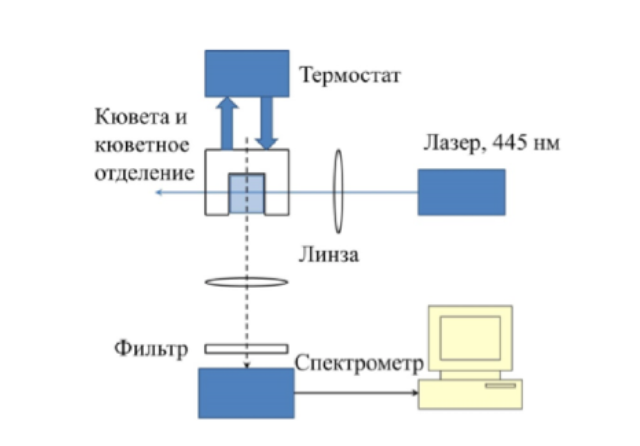
\includegraphics[width=0.8\linewidth]{Images/схема.png}
    \caption{Схема установки}
    \label{fig: схема}
\end{figure}
\section{Результаты и обсуждение}\;
\subsection{Измерение параметров установки}
\par Для оценки параметров прибора мы сняли спектр изопропанола при $\lambda = 445$ нм (рис. \ref{fig:наш}). 
\begin{figure}[h!]
\centering
    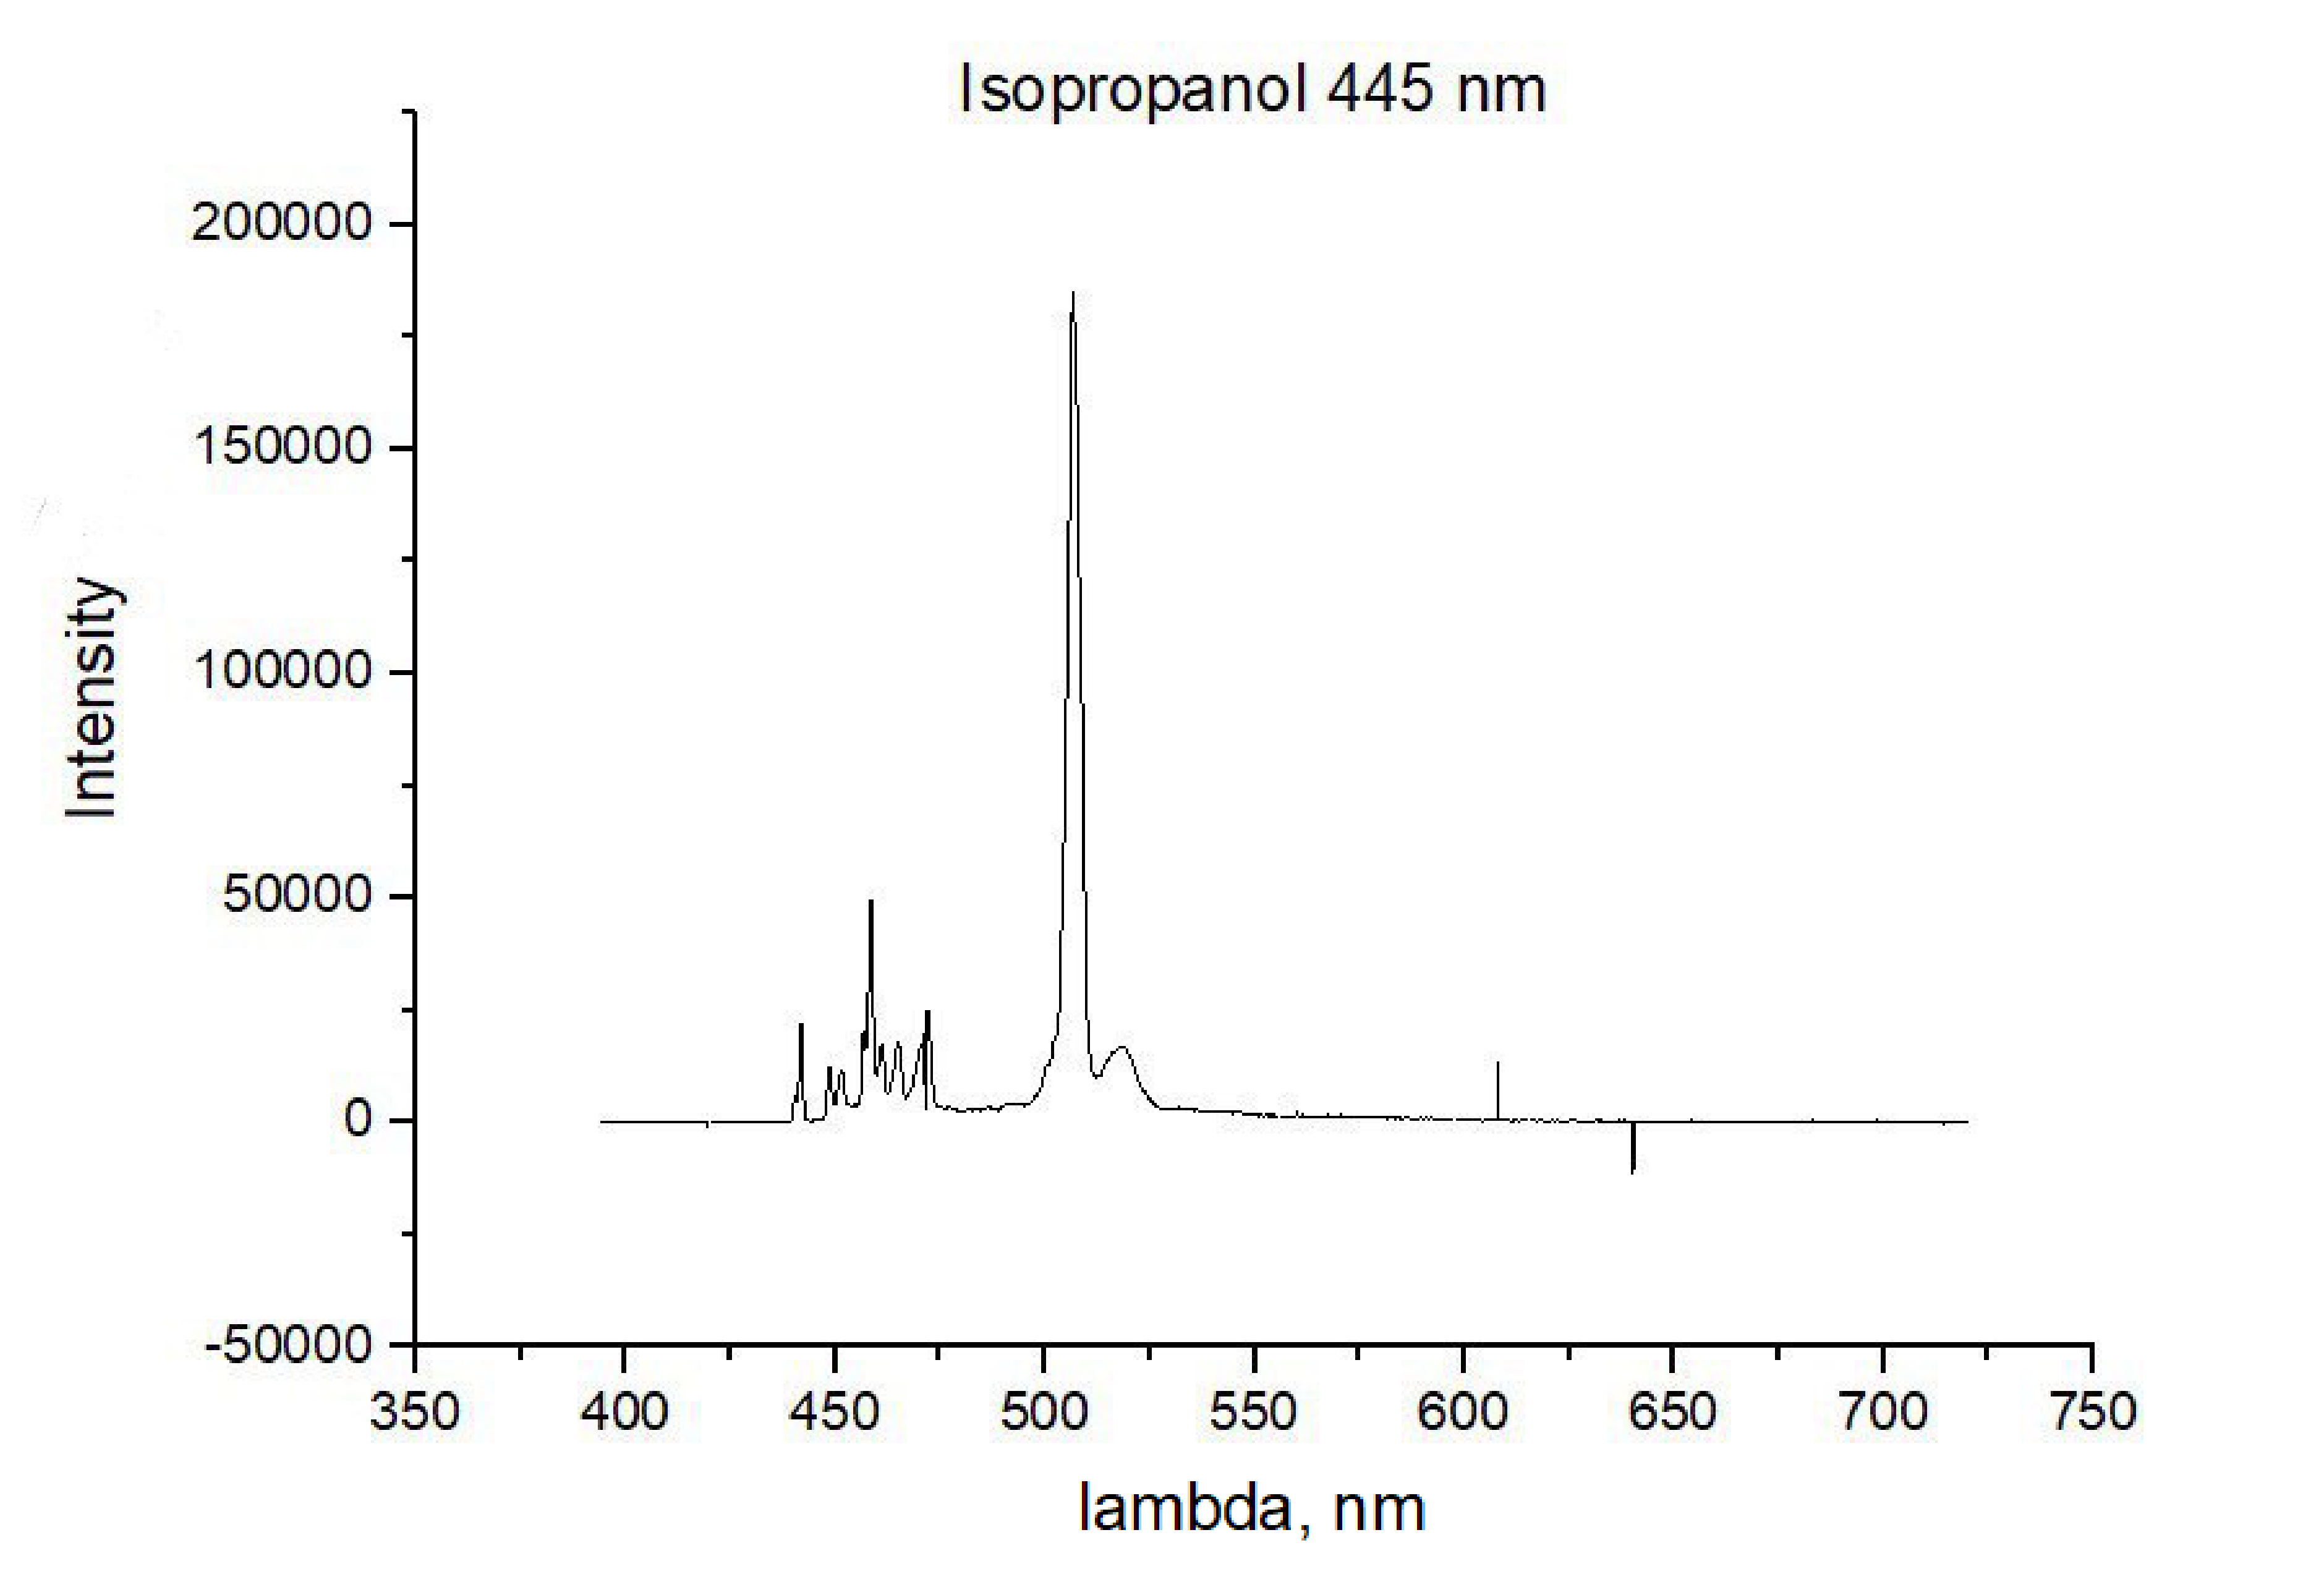
\includegraphics[width=0.8\linewidth]{Images/iso 445.png}
    \caption{Наш спектр изопропанола при 445 нм}
    \label{fig:наш}
\end{figure}
\par Рассмотрим два левых пика (рис. \ref{fig:наш}):
$$\lambda = 5487 \text{A}$$
$$\lambda + \delta \lambda = 5516 \text{A}$$
$$R = \frac{\lambda}{\delta \lambda} = \frac{\lambda _1}{\lambda _2 - \lambda _1} = 189,2 \text{A}$$
\par А теперь рассмотрим эталонный спектр (рис.\ref{red}), полученный на другой установке:
\begin{figure}[h!]
\centering
    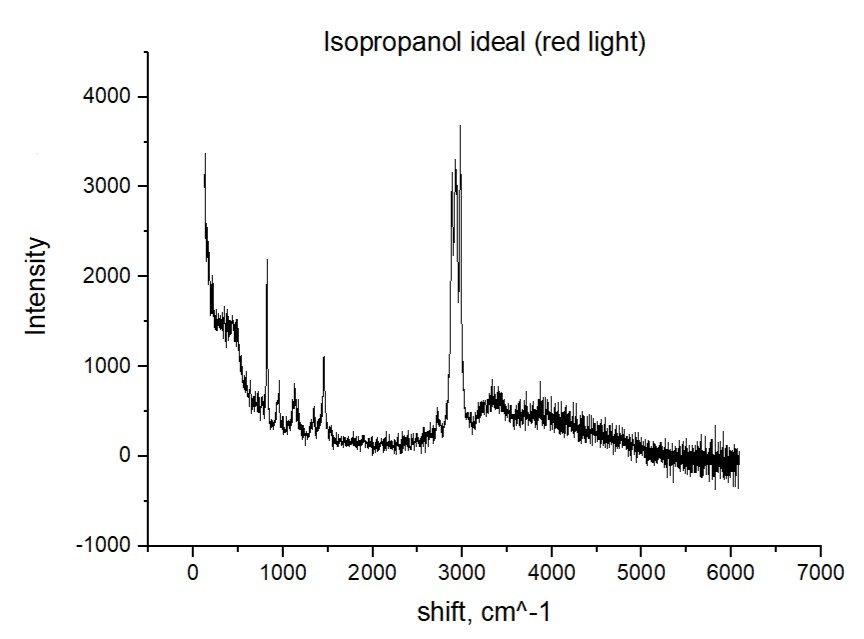
\includegraphics[width=0.8\linewidth]{Images/iso.jpg}
    \caption{Эталонный спектр изопропанола, полученный с другой установки с красным излучением}
    \label{red}
\end{figure}
\newpage
\par На спектре чётко различаются следующие пики: пик на
$ \approx 800 \text{см}^{-1}$ – это связь C-C, пик на $ \approx 1100 \text{см}^{-1}$
- связь C-O, пик на $ \approx 1500 \text{см}^{-1}$ – деформационные колебания, а пики на $ \approx 2880 , 2920 \text{ и } 2970 \text{см}^{-1}$ – валентные колебания $\text{C-CH}_3$ и C-H.
\par Для корректного сравнения пиков перейдём от нм к сдвигу (shift) в $\text{см}^{-1}$ (рис. \ref{shift}) с помощью следующей формулы:
$$\text{shift} = \frac{1}{\lambda _0} - \frac{1}{\lambda}$$
\begin{figure}[h!]
\centering
    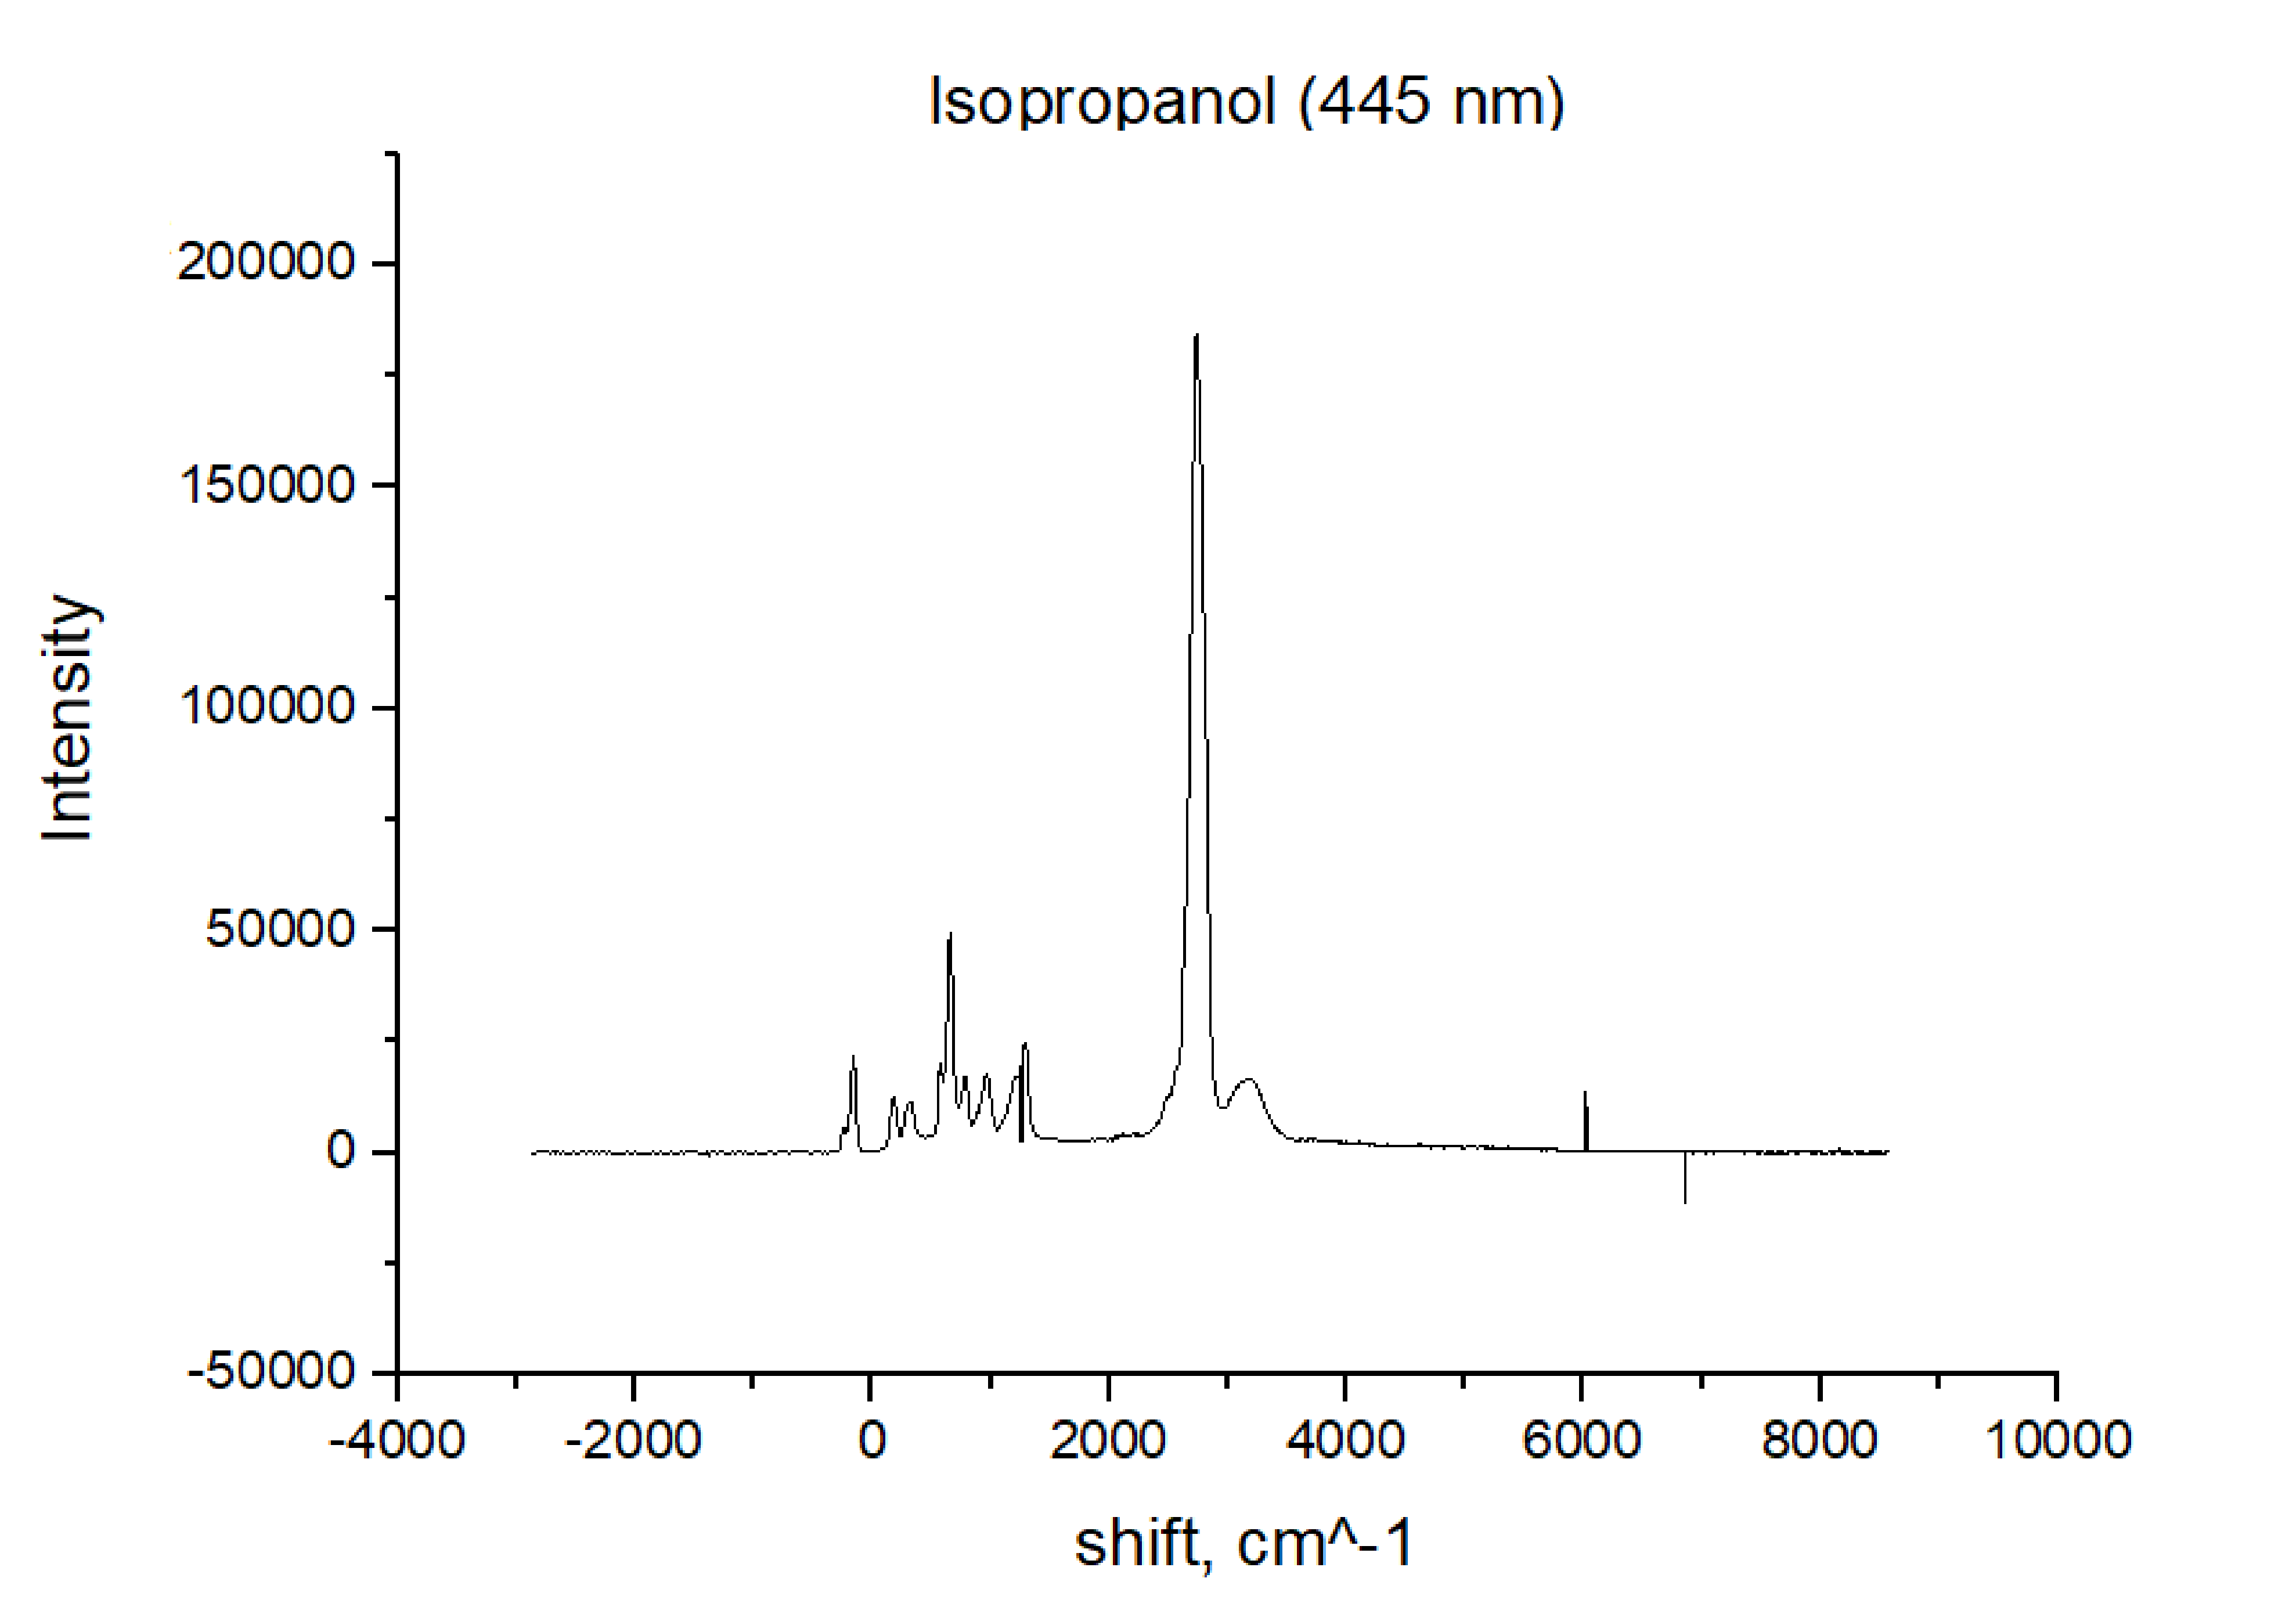
\includegraphics[width=0.8\linewidth]{Images/iso 445 shift.png}
    \caption{Наш спектр изопропанола в координатах рамановского сдвига}
    \label{shift}
\end{figure}
\par Тогда результаты представим в виде таблицы (таблица \ref{tab:my-table}):

\begin{table}[h!]
\centering
\begin{tabular}{|l|l|}
\hline
Спектр при 445 нм, $\text{см}^{-1}$ & Эталонный спектр, $\text{см}^{-1}$ \\ \hline
не разрешён                    & 2976             \\ \hline
не разрешён                    & 2927             \\ \hline
не разрешён                     & 2880             \\ \hline
    1319          & 1468             \\ \hline
    1140          & 1145             \\ \hline
    673         & 856              \\ \hline
\end{tabular}
\caption{Сравнение пиков для спектра, полученного во время лабораторной работы, и эталонного}
\label{tab:my-table}
\end{table}
\par Представим также спектр изопропанола, полученный на той же установке, но с зелёным лазером с $\lambda$ = 532 нм (рис. \ref{532nm}):
\begin{figure}[h!]
\centering
    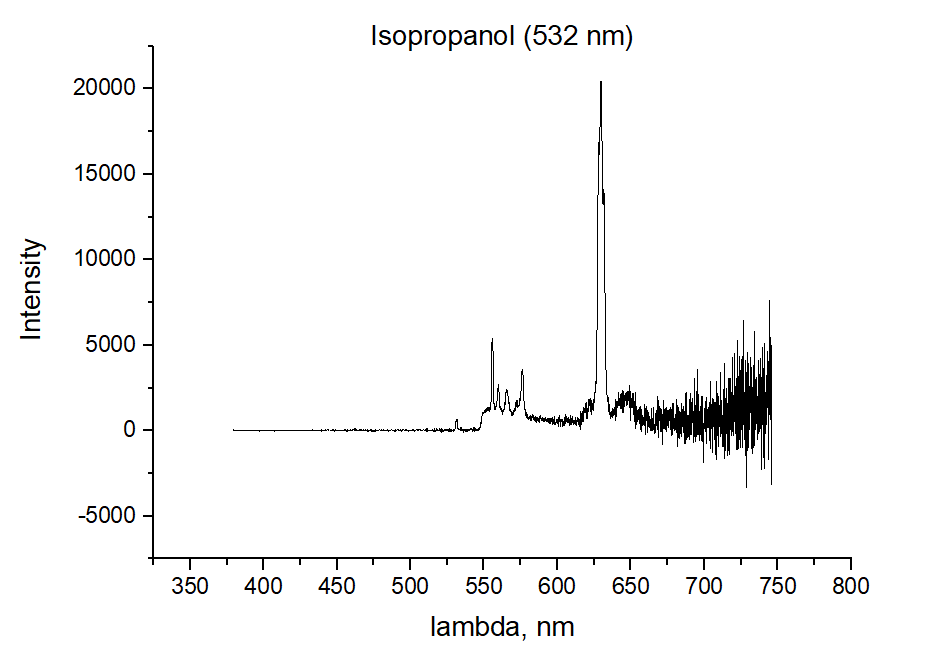
\includegraphics[width=0.8\linewidth]{Images/iso 532.png}
    \caption{Спектр изопропанола при 532 нм}
    \label{532nm}
\end{figure}
\par Если сравнить этот спектр с полученным нами при $\lambda = 445$ нм (рис. \ref{fig:наш}), то можно сделать вывод, что форма спектра не зависит от длины волны, только от характеристик исследуемого вещества. Изменяется только амплитуда пика, так как рамановское сечение пропорционально $\frac{1}{\lambda ^4}$.
\par Рассмотрим как поляризация в вертикальном (рис. \ref{вертикаль}) и горизонтальном направлении (рис. \ref{горизонталь}) повлияли на спектр изопропанола с $\lambda$ = 445 нм:
\begin{figure}[h!] 
        \centering
        \minipage{0.5\textwidth}
        \centering
            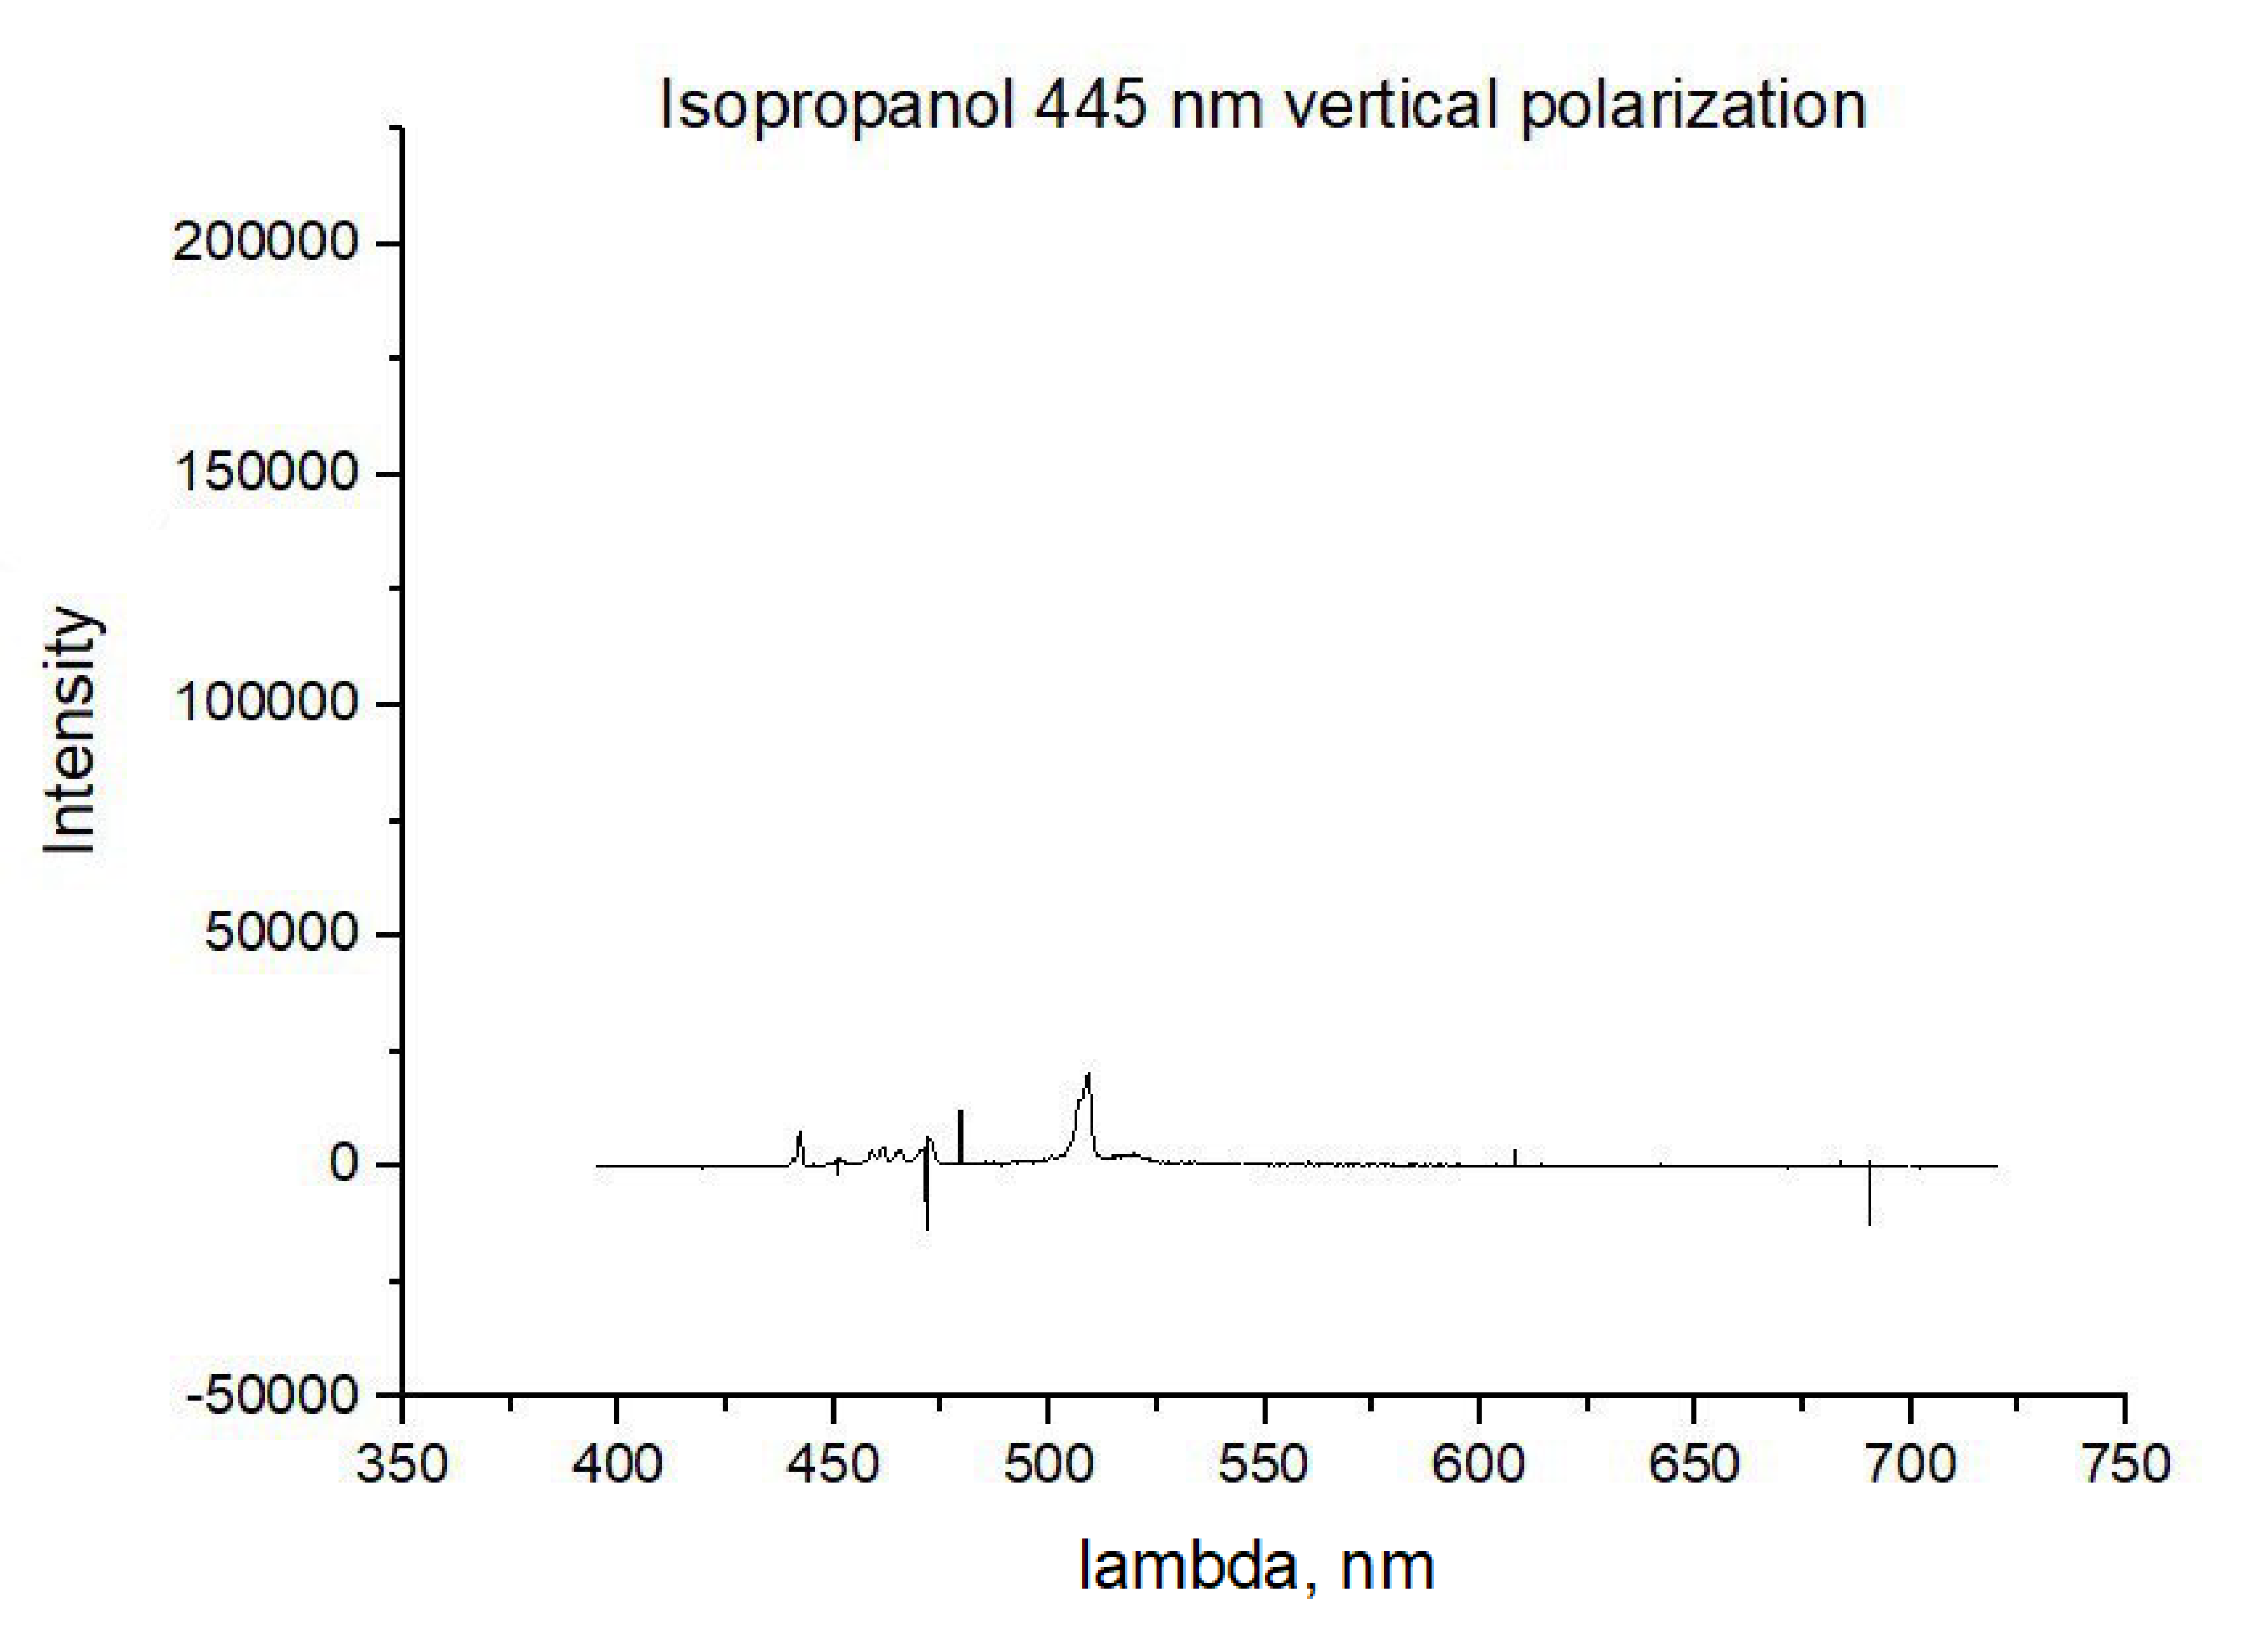
\includegraphics[width=0.8\linewidth]{Images/вертикаль.png}
                 \caption{Спектр с вертикальной поляризацией}
                 \label{вертикаль}
        \endminipage\hfill
        \minipage{0.5\textwidth}
        \centering
             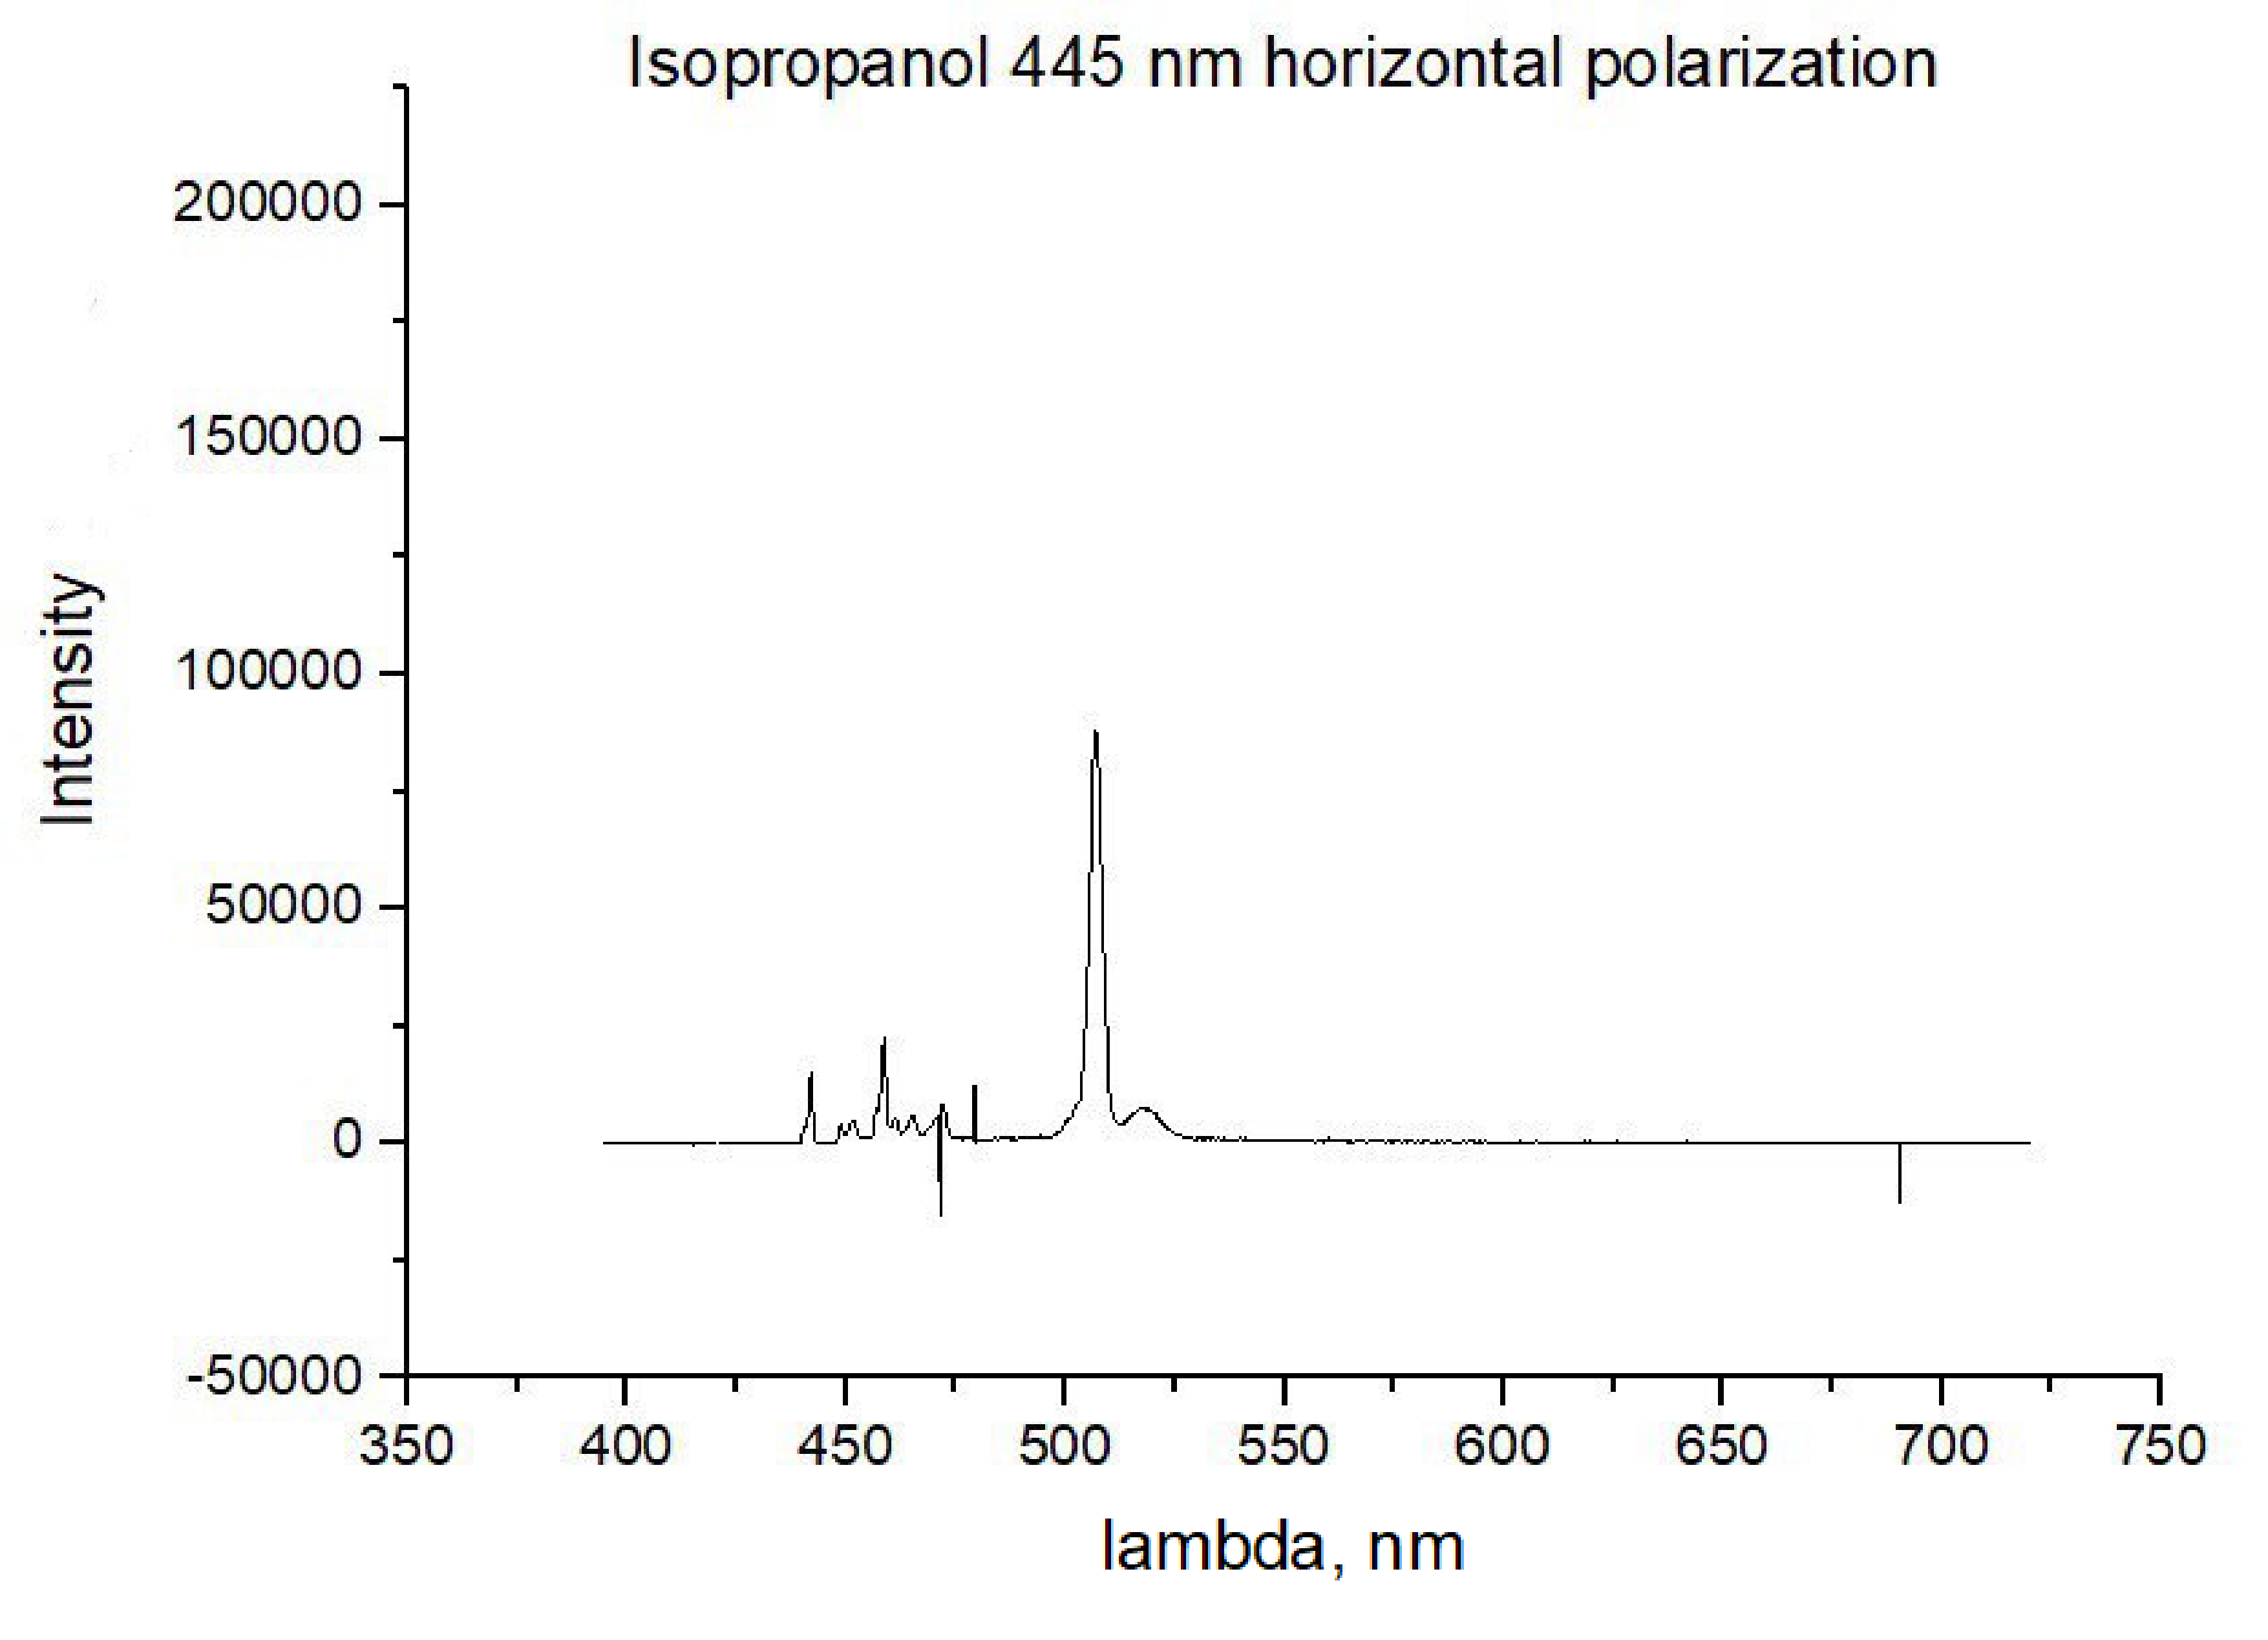
\includegraphics[width=0.8\linewidth]{Images/горизонталь.png}
                 \caption{Спектр с горизонтальной поляризацией}
                 \label{горизонталь}
        \endminipage
\end{figure}
\par При горизонтальной поляризации форма спектра остаётся неизменной, но падает интенсивность примерно в 2 раза, что соответствует прохождению через поляроид. А в случае вертикальной поляризации практически весь главный пик отсекается на пластинке и не проходит через поляроид.

\newpage

\subsection{Получение спектров комбинационного рассеяния воды}
\subsubsection{Снятие спектра воды при комнатной температуре}\;

\par В начале данной части работы снимем спектр КРС воды при комнатной температуре ($T = 20,5 \; ^{\circ}C$), который приведён на Рис. \ref{Вода, комната}. При детальном рассмотрении можно отметить, что основные два пика спектра имеют рамановский сдвиг $3129,05\; \text{см}^{-1}$ и $3258,79\; \text{см}^{-1}$. Эти два пика отвечают полимерным и мономерным структурам воды (соотношения площадей под пиками будут давать информацию о температурной зависимости количества водородных связей в растворе).

\begin{figure}[h!]
\centering
    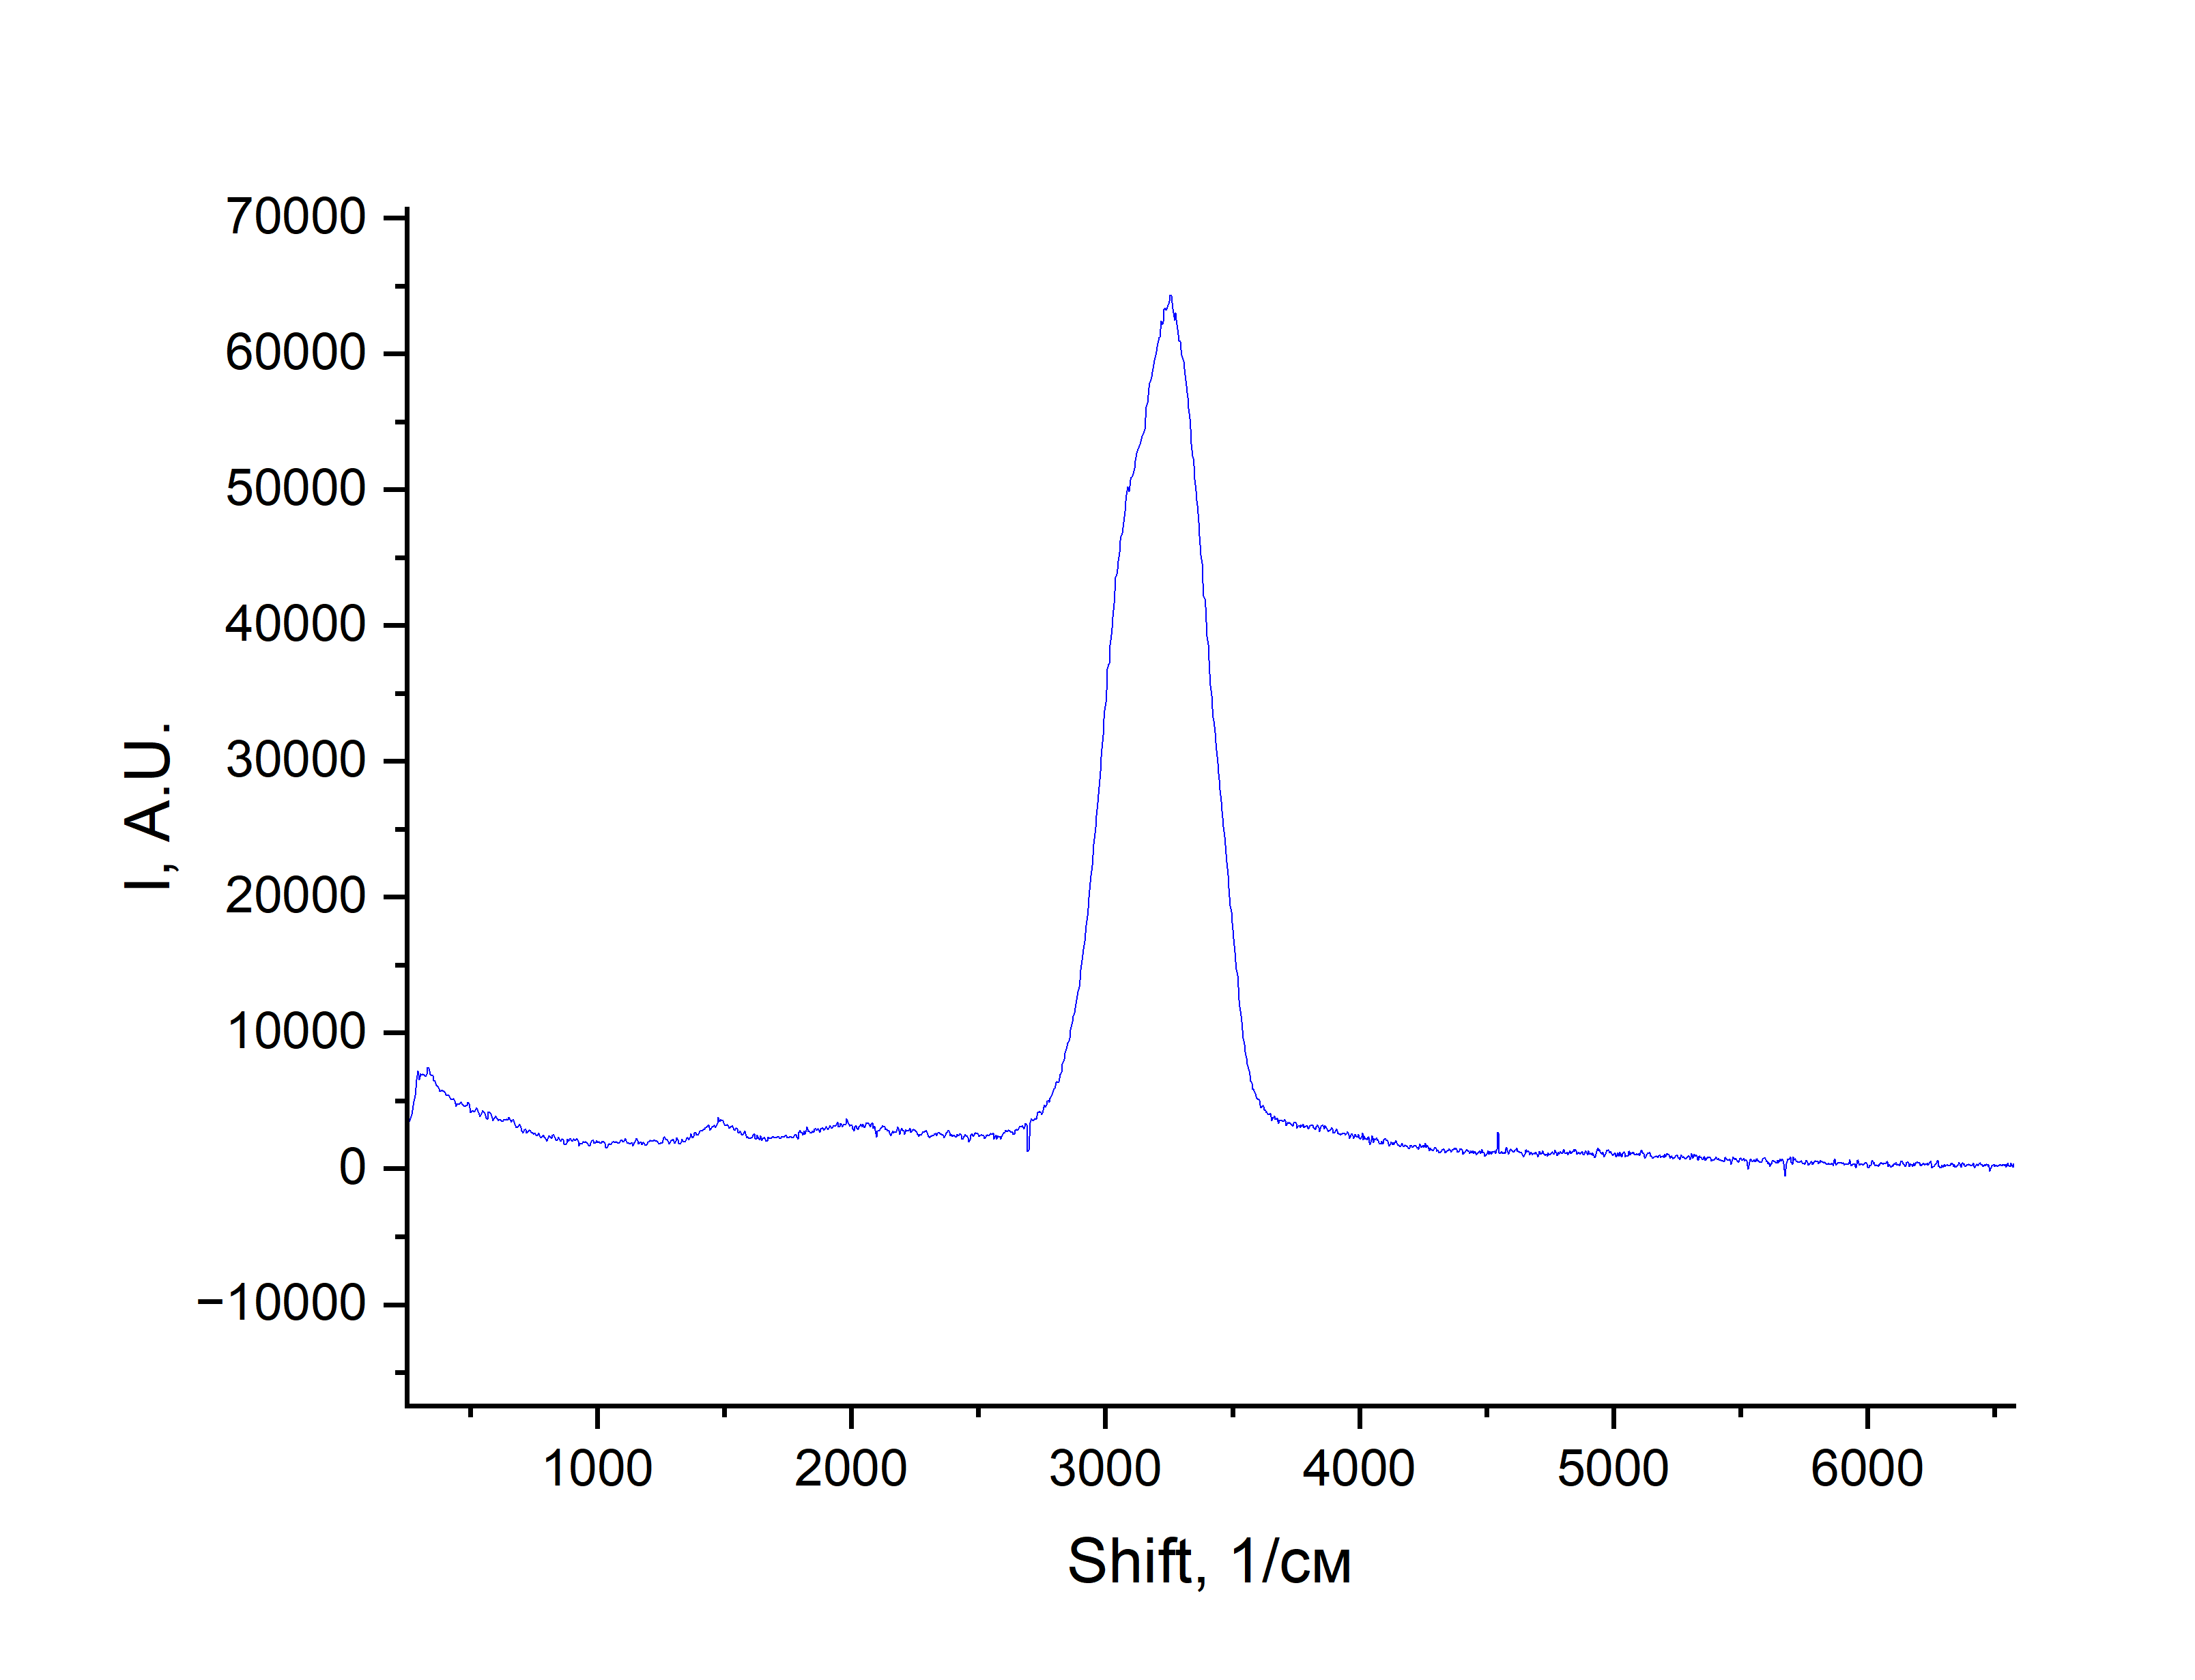
\includegraphics[width=0.6\linewidth]{Images/Вода; комнатная температура.png}
    \caption{Рамановский спектр воды ($T = 20,5 \; ^{\circ}C$).}
    \label{Вода, комната}
\end{figure}


\subsubsection{Сравнение спектров КРС для лазеров с разными длинами волн}\;

\par В работе предлагается сравнить между собой спектры воды при $T = 30 \; ^{\circ}C$, снятых лазерами $\lambda_1 = 445 \; \text{нм}$ и $\lambda_2 = 532 \; \text{нм}$ (Рис. \ref{Вода, сравнение}). По данному рисунку можно отметить, что положения пиков практически не изменились при изменении длины волны (1: $3100 - 3200 \; \text{см}^{-1}, \; 2: 3300 - 3400 \; \text{см}^{-1}$). Однако для более длинноволнового лазера интенсивность рассеяния много ниже, чем для используемого в работе. Таким образом, это визуальное расположение лишний раз подтверждает зависимость интенсивности рассеяния от длины волны.

\begin{figure}[h!]
\centering
    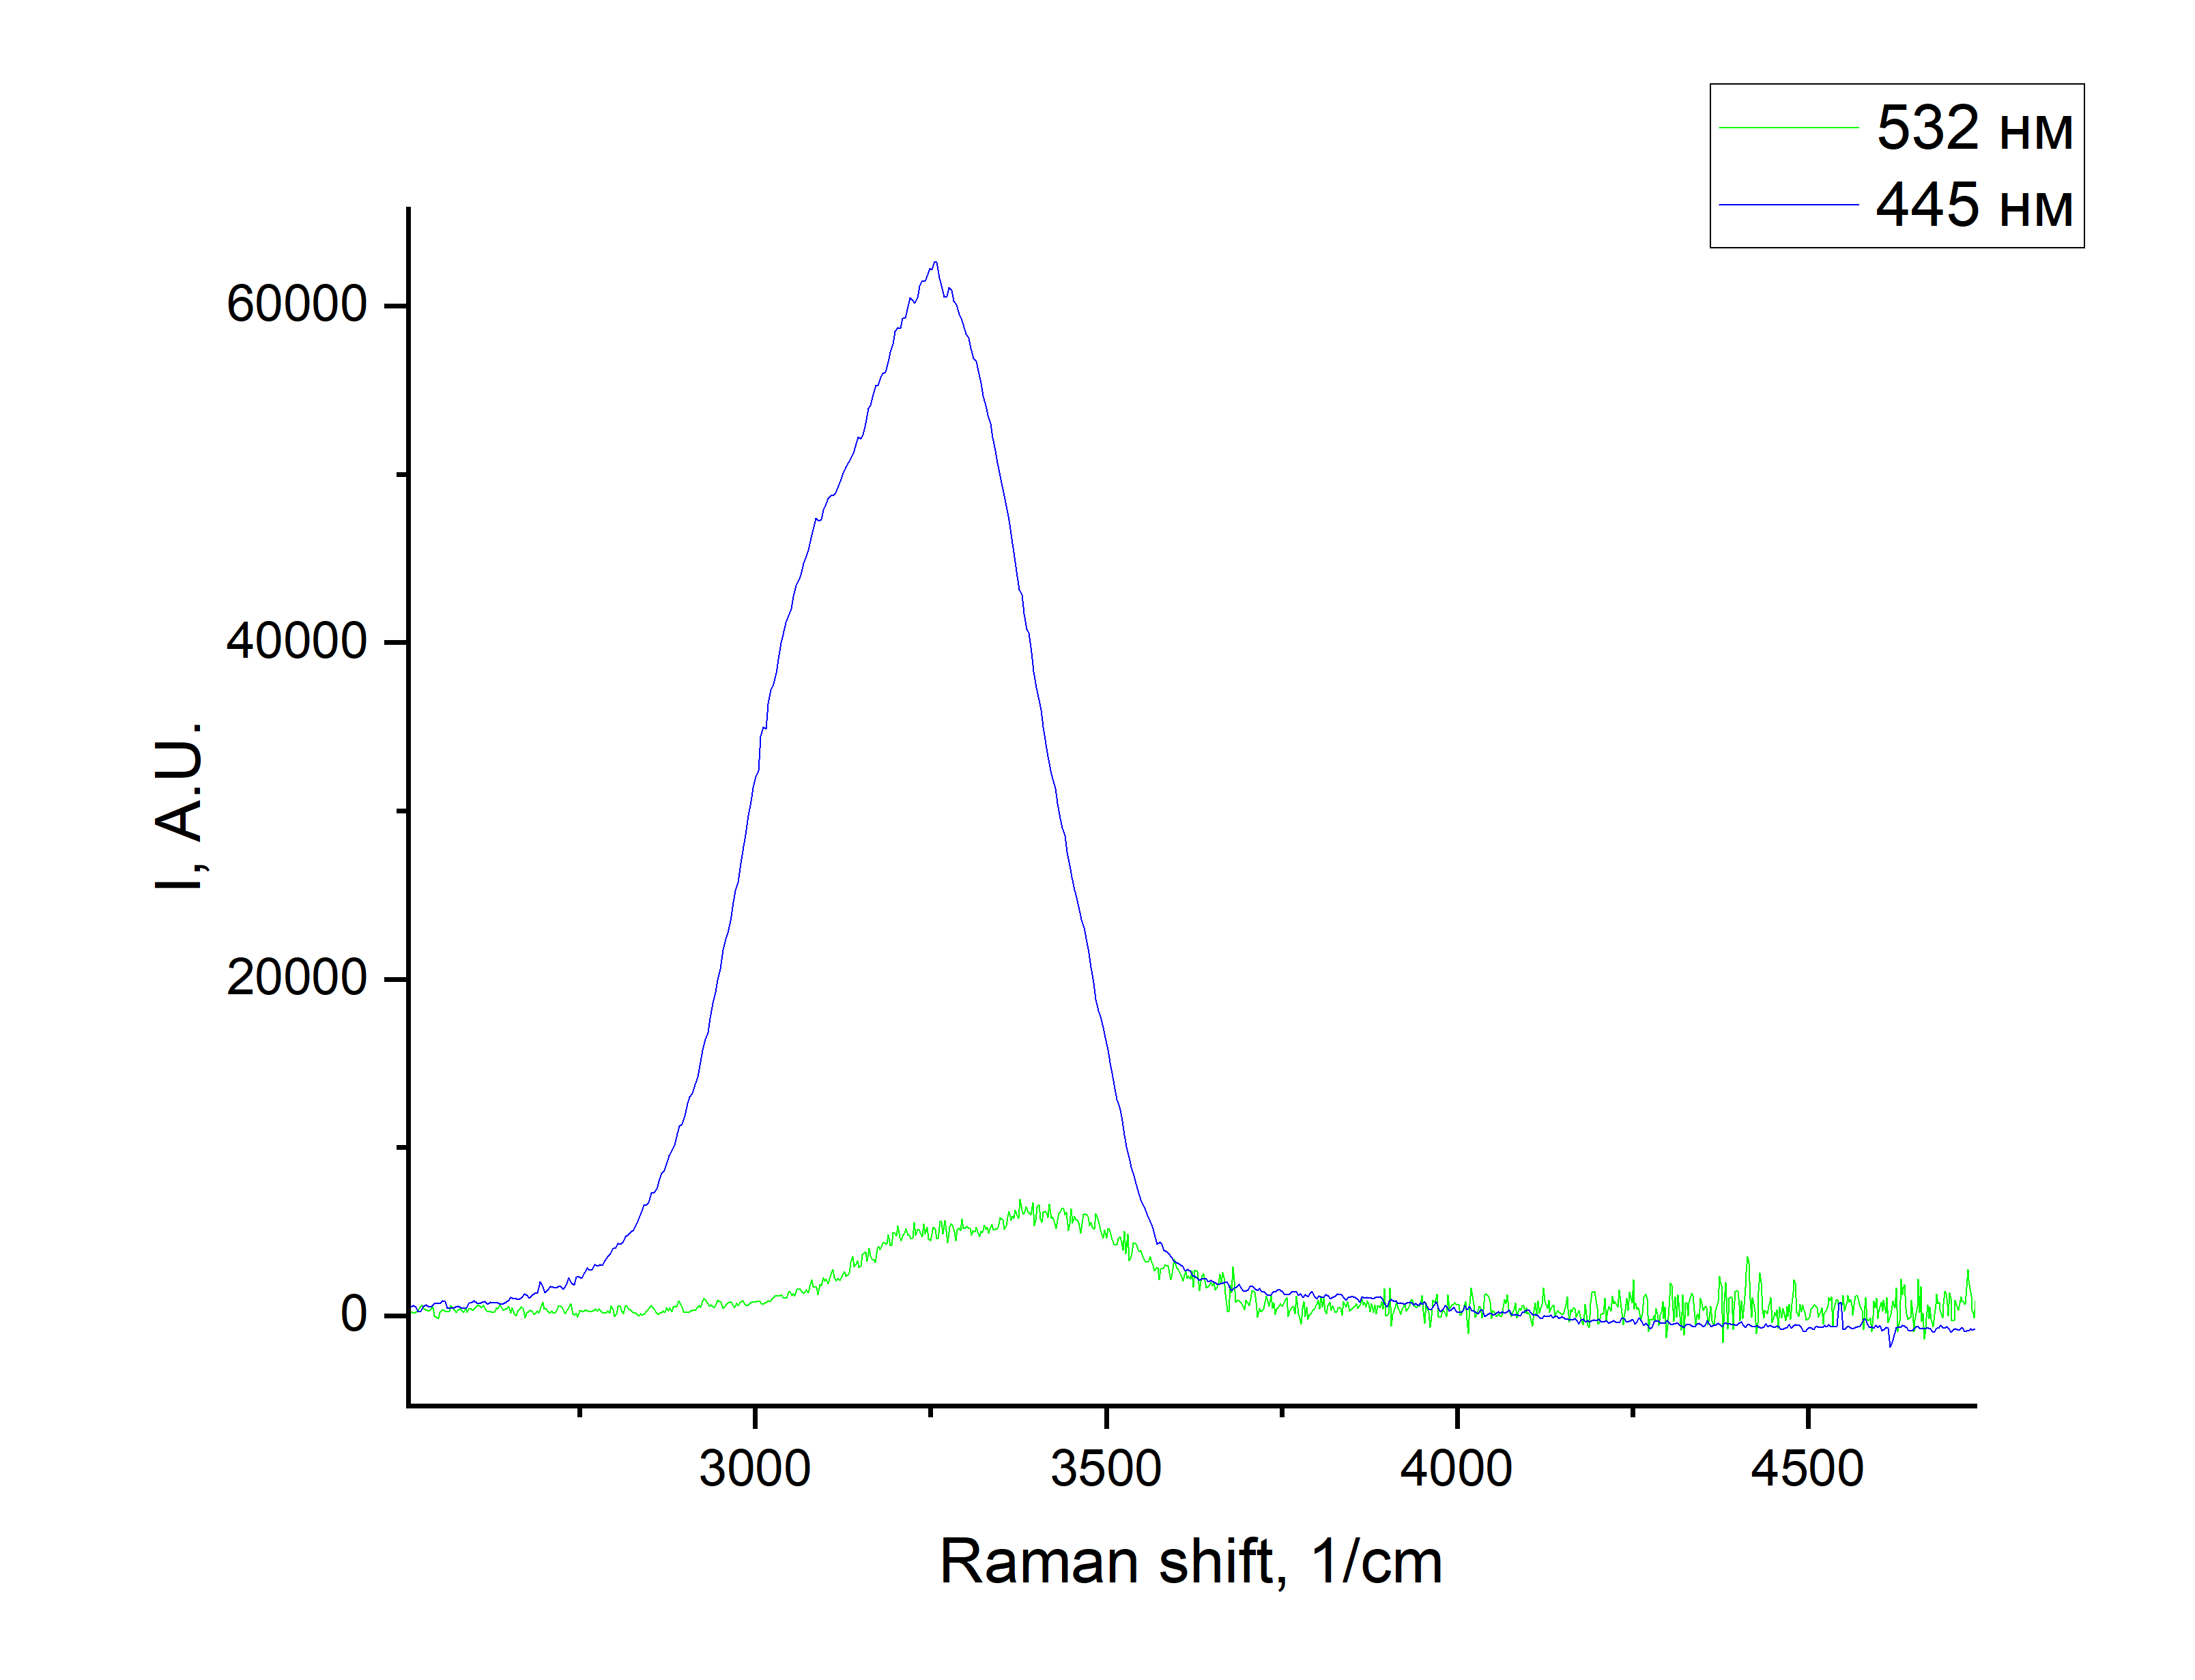
\includegraphics[width=0.6\linewidth]{Images/Вода; сравнение лазеров.png}
    \caption{Рамановский спектры воды ($T = 30 \; ^{\circ}C$) при облучении лазерами с разными длинами волн.}
    \label{Вода, сравнение}
\end{figure}

\subsubsection{Сравнение спектров КРС при разных положениях поляризатора}\;

\par Поставим на пути лазера поляризатор в двух положениях: когда разрешённое положение поляроида совпадает с ориентацией поляризованного света из лазера и когда они находятся в скрещенном состоянии. Результаты снятия спектров КРС представлены на Рис. \ref{Вода, поляризация}.

\begin{figure}[h!]
\centering
    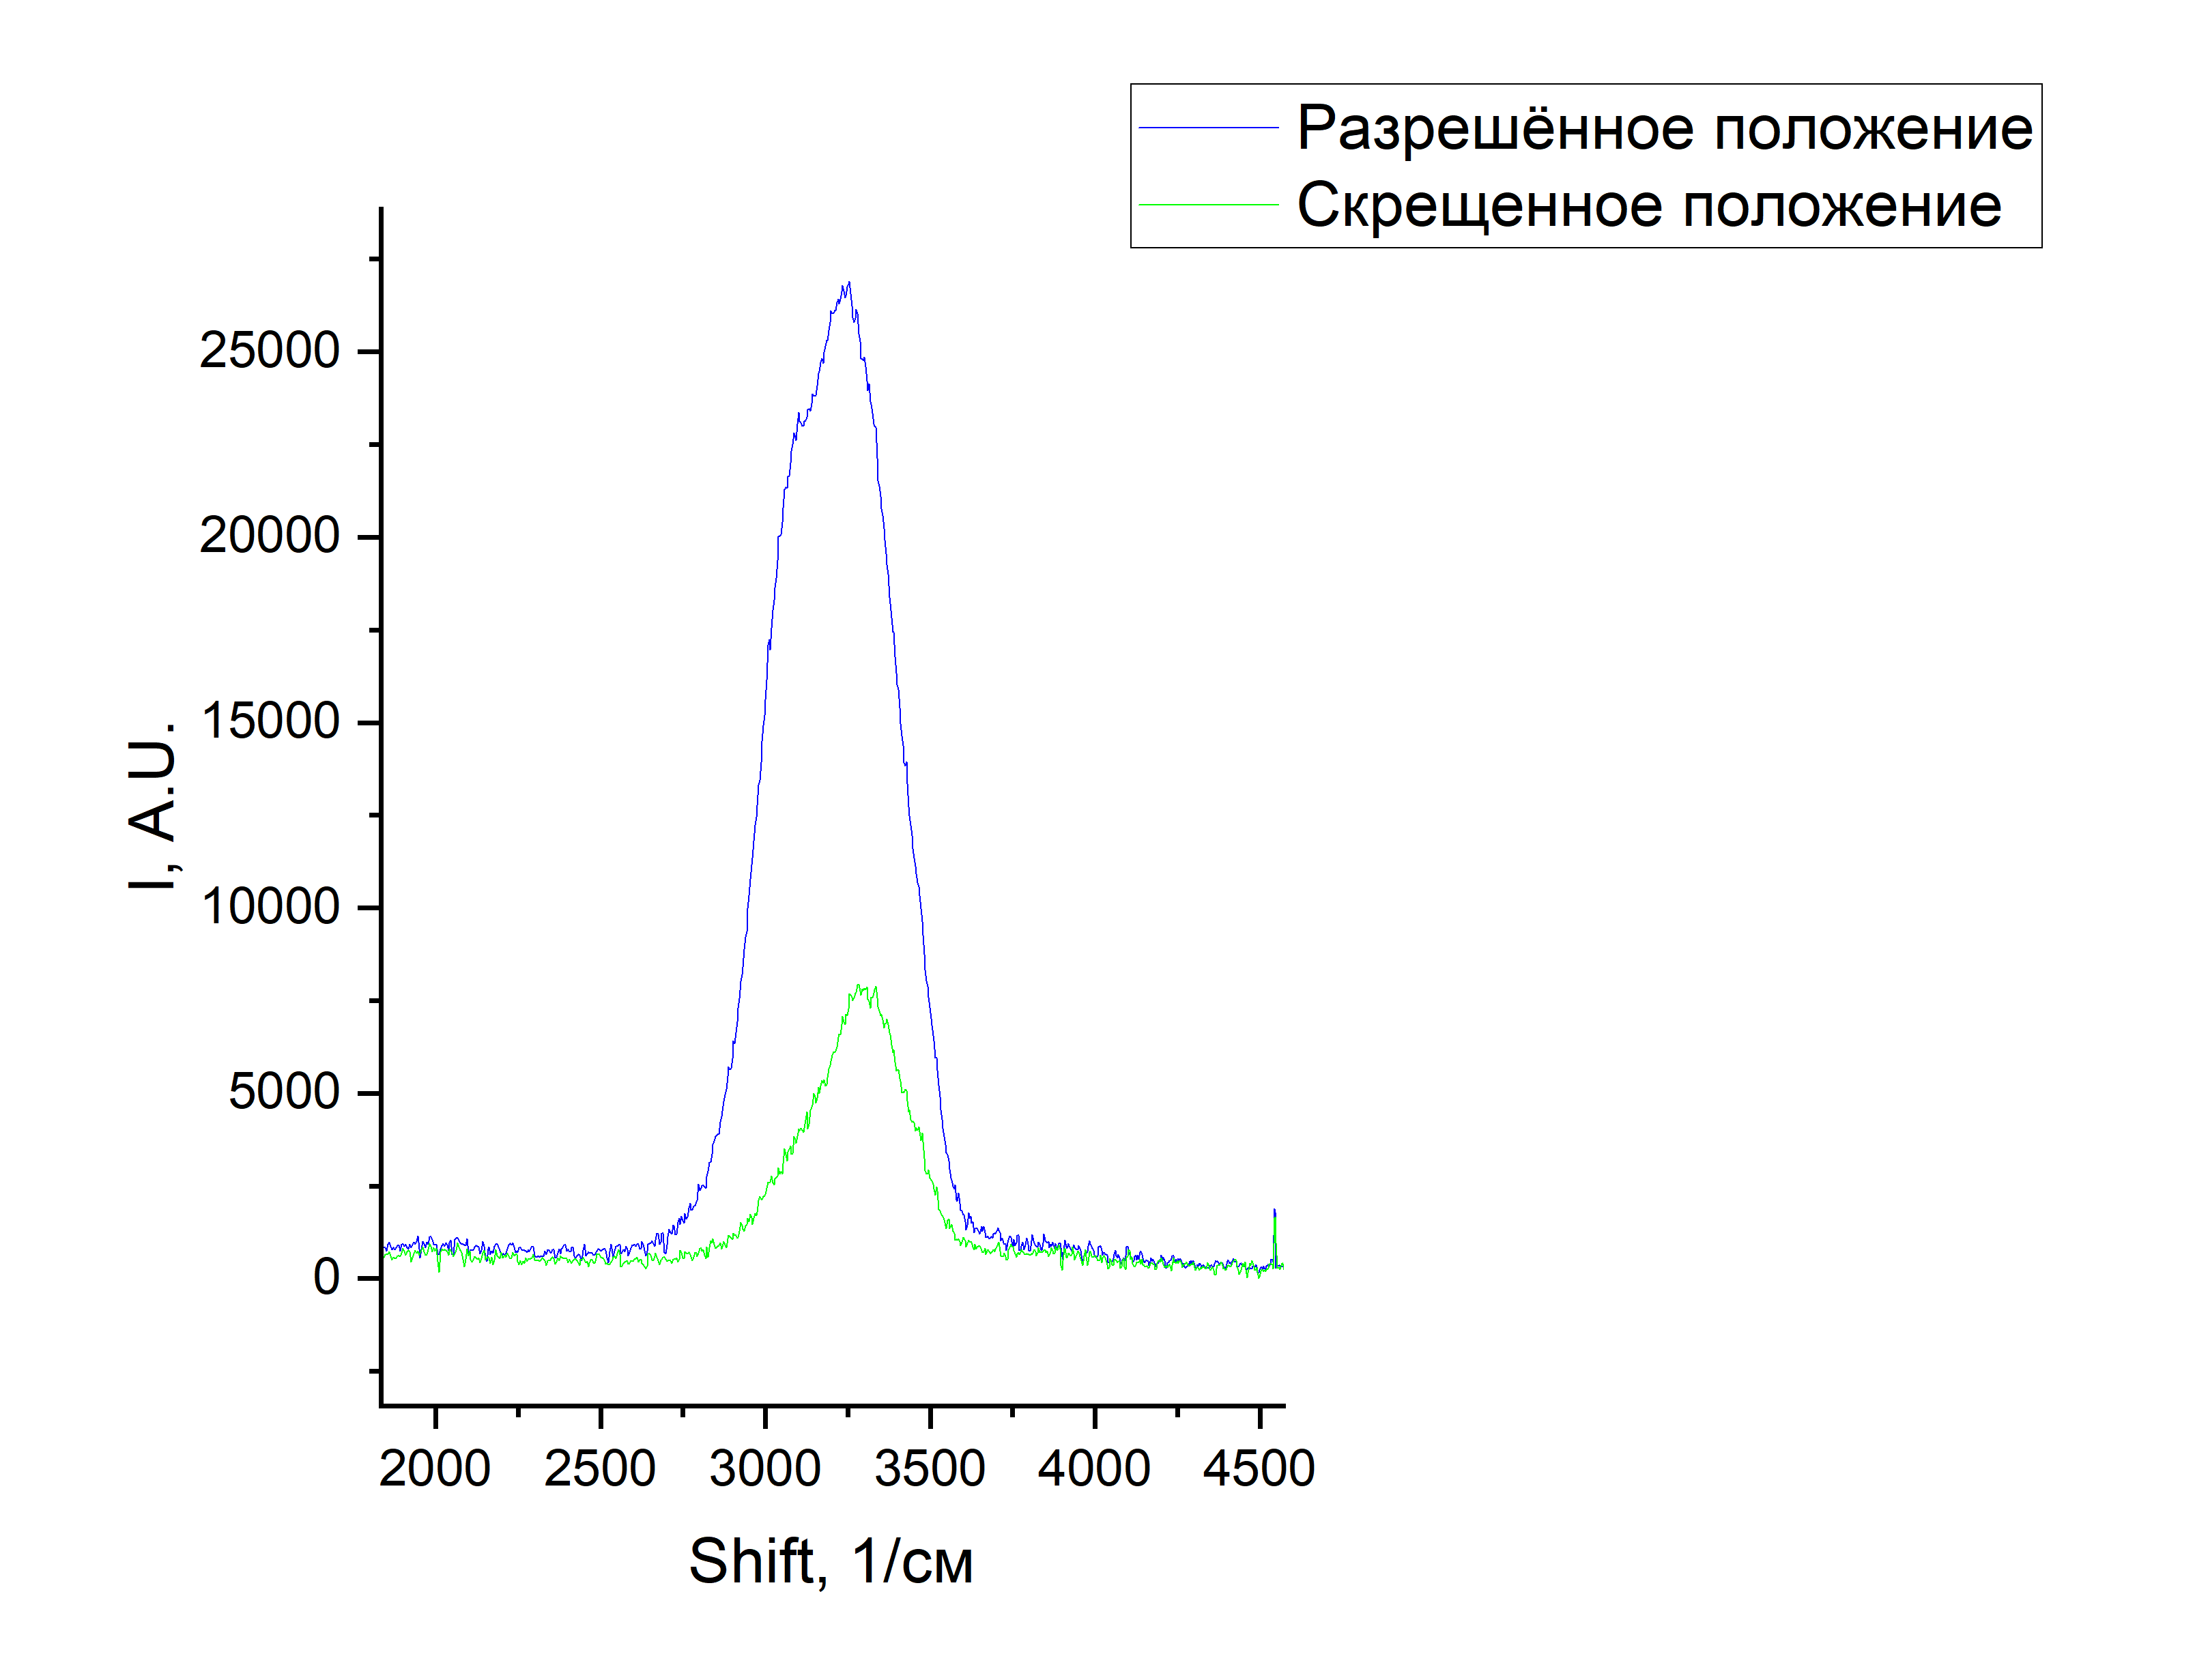
\includegraphics[width=0.6\linewidth]{Images/Вода; сравнение поляризаций.png}
    \caption{Спектры КРС воды ($T = 20,5 \; ^{\circ}C$) при разных положениях поляризатора}
    \label{Вода, поляризация}
\end{figure}

На приведённом рисунке можно отметить разность интенсивностей при приблизительном сохранении положения пиков на оси абсцисс. 

\subsubsection{Нахождение средней энергии водородной связи в растворе}\;

\par В данной части работы предлагается посредством изменения температуры и снятия спектров КРС пронаблюдать изменение формы пиков. На основании декомпозиции пиков определить соотношение молекул-мономеров и полимеров. 

\par Для получения средней энергии водородной связи нужно использовать следующие выкладки. Представим реакции образования водородных связей в растворе, как химическую реакцию превращения мономеров в полимеры.

$$M \rightleftarrows P$$

\par Как и любая химическая реакция, она обладает константой равновесия, которую можно выразить двумя способами:

$$k = \frac{[P]}{[M]} = \frac{I_P}{I_M}$$
$$\frac{\partial \ln{k}}{\partial T} = - \frac{Q}{RT^2}$$

\par Приводя математические преобразования получаем следующее:
$$d \ln{k} = \frac{Q}{R}d \left(\frac{1}{T}\right)$$

\par Следовательно, наклон графика $\ln{k}\left(\frac{1}{T}\right)$ будет представлять отношение теплового эффекта реакции к газовой постоянной.

\par Путём декомпозиции (приведены в Приложении) получим следующие данные, которые занесём в Таблицу \ref{Вода}.

\begin{table}[h!]
\centering
\caption{Данные для расчёта энергии водородной связи}
\begin{tabular}{|l|l|l|}
\hline
$T, ^{\circ}C$ & $\frac{1}{T}, \frac{1}{K}$ & $\ln{\frac{I_P}{I_M}}$ \\ \hline
20,5 & 0,00341 & -0,837 \\ \hline
30 & 0,00330 & -0,870 \\ \hline
40 & 0,00319 & -0,892 \\ \hline
51 & 0,00309 & -1,178 \\ \hline
60,2 & 0,00300 & -1,027 \\ \hline
69,6 & 0,00292 & -1,253 \\ \hline
79,4 & 0,00284 & -1,372 \\ \hline
\end{tabular}
\label{Вода}
\end{table}


На основании полученных значений построим зависимость $\ln{\frac{I_P}{I_M}}\left(\frac{1}{T}\right)$. Полученный график приведён на Рис. \ref{Водородная связь}.

\begin{figure}[h!]
\centering
    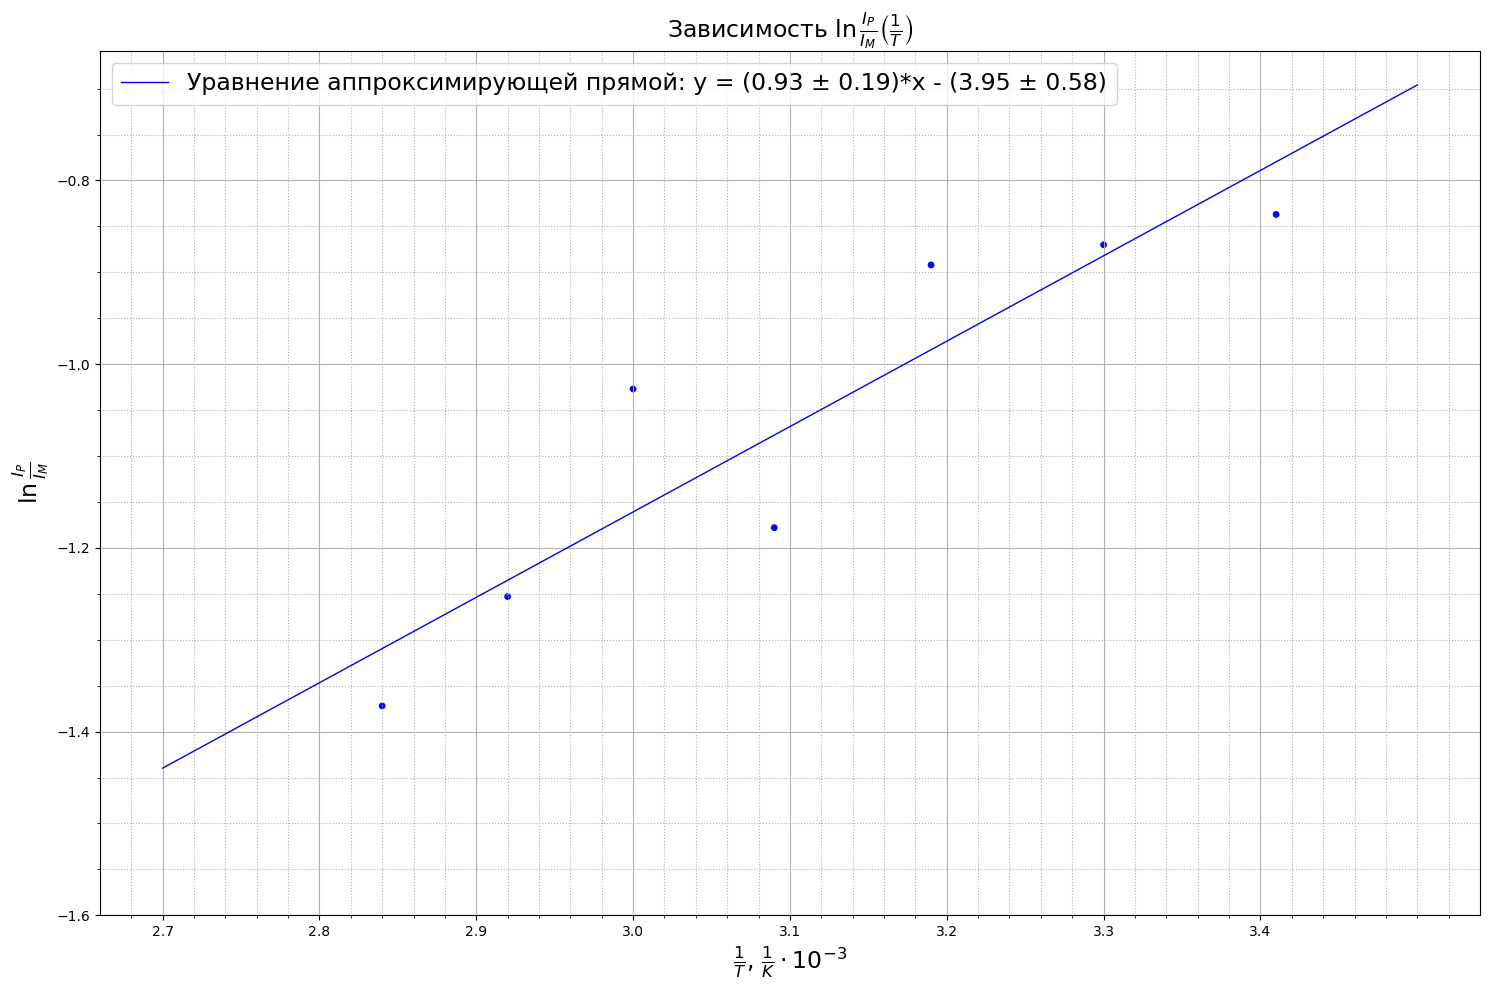
\includegraphics[width=0.7\linewidth]{Images/Нафиг график.png}
    \caption{Зависимость $\ln{\frac{I_P}{I_M}}\left(\frac{1}{T}\right)$}
    \label{Водородная связь}
\end{figure}


Из коэффициента наклона и погрешности аппроксимации получаем:
$$E = (7,7 \pm 1,6) \; \frac{\text{кДж}}{\text{моль}}$$
\section{Выводы}
\begin{enumerate}
    \item Из спектра изопропанола определили разрешающую способность установки:
    $$R = 189,2 \text{A}$$
    \item Определили, что форма спектра не зависит от длины волны излучения, а только от характеристик исследуемого вещества.
    \item Изменение формы спектра происходило только при вертикальной поляризации, при которой практически полностью отсекался основной пик. При горизонтальной поляризации уменьшалась только интенсивность примерно в 2 раза.
    \item При изучении спектров КРС воды была так же показана независимость положения пиков от длины волны лазера и положения поляризатора на пути пука света (эти параметры влияют только на интенсивность рассеяния).
    \item При исследовании температурной зависимости спектров КРС воды была оценена энергия водородной связи в растворе:
    $$E = (7,7 \pm 1,6) \; \frac{\text{кДж}}{\text{моль}}, \; \varepsilon = 20,8 \%$$
    При этом реальное значение энергии водородной связи в воде оценивается в $20,9 \; \frac{\text{кДж}}{\text{моль}}$.
\end{enumerate}
\section{Приложение}
\begin{figure}[!htb]
                \minipage{0.45\textwidth}
                 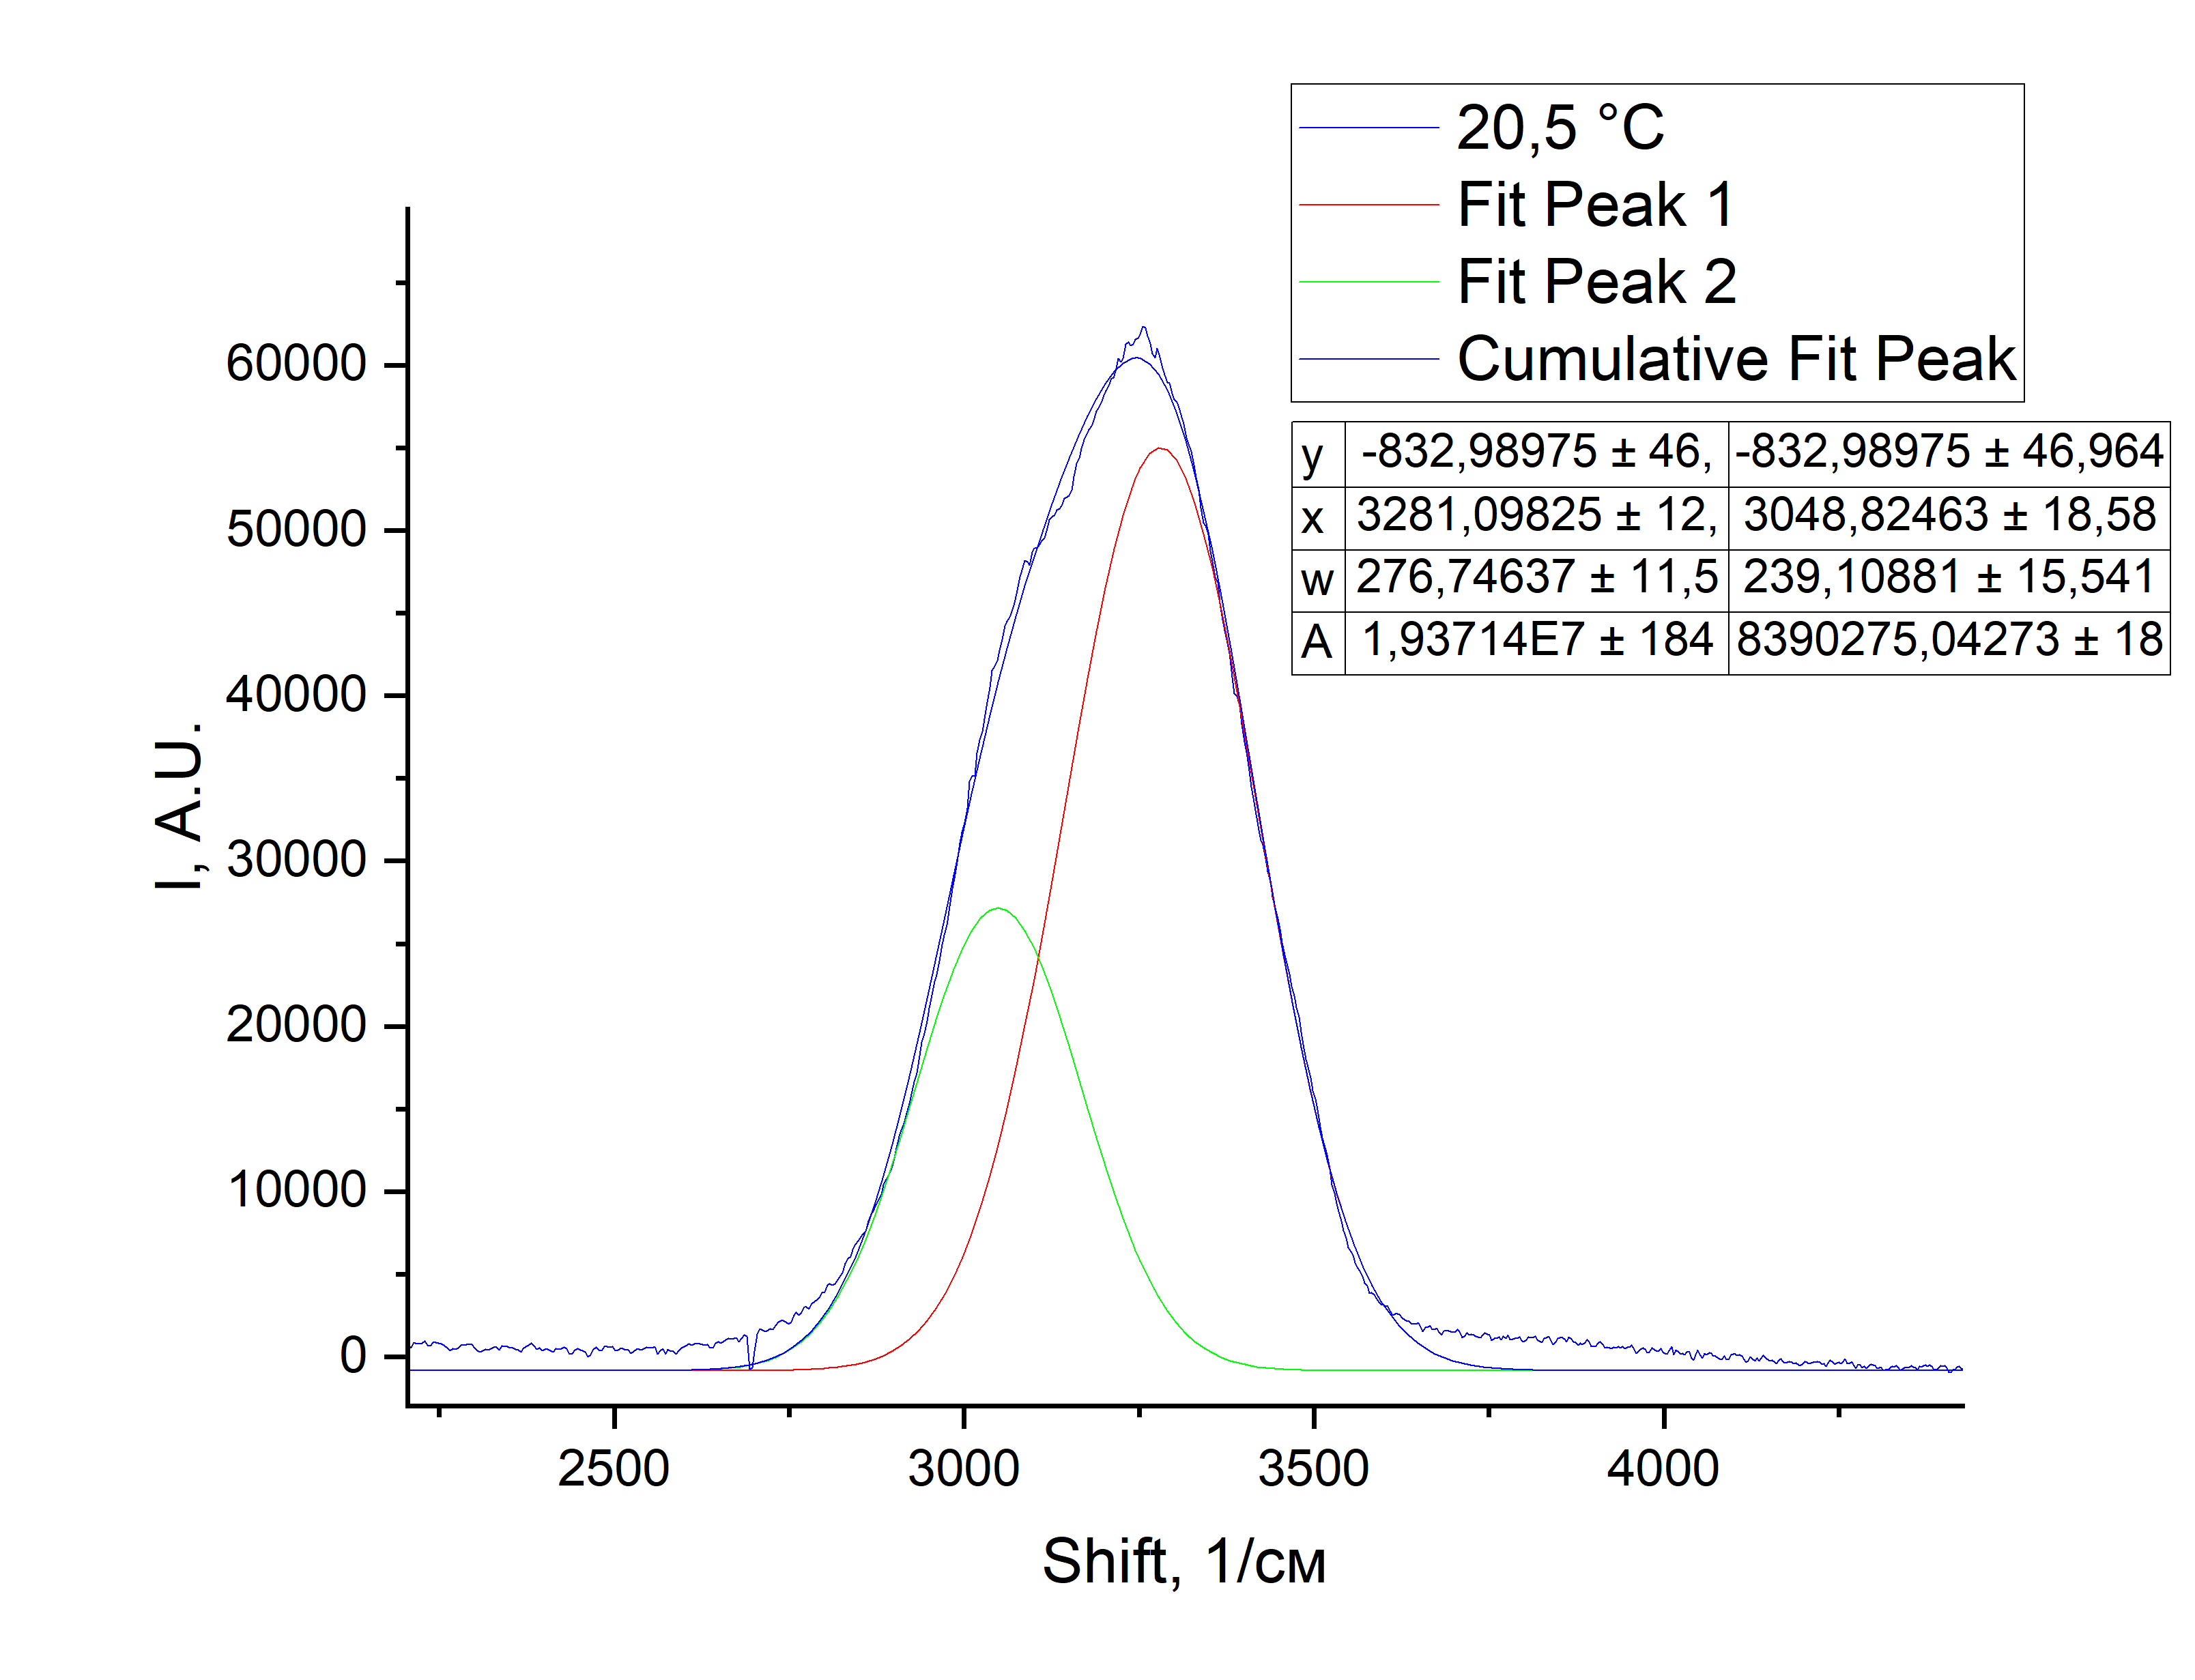
\includegraphics[width=\linewidth]{Images/Вода; 20.png}
                 \caption{Декомпозиция спектра КРС воды для $T = 20,5 \; ^{\circ}C$}
                  \endminipage\hfill
                \minipage{0.45\textwidth}
                 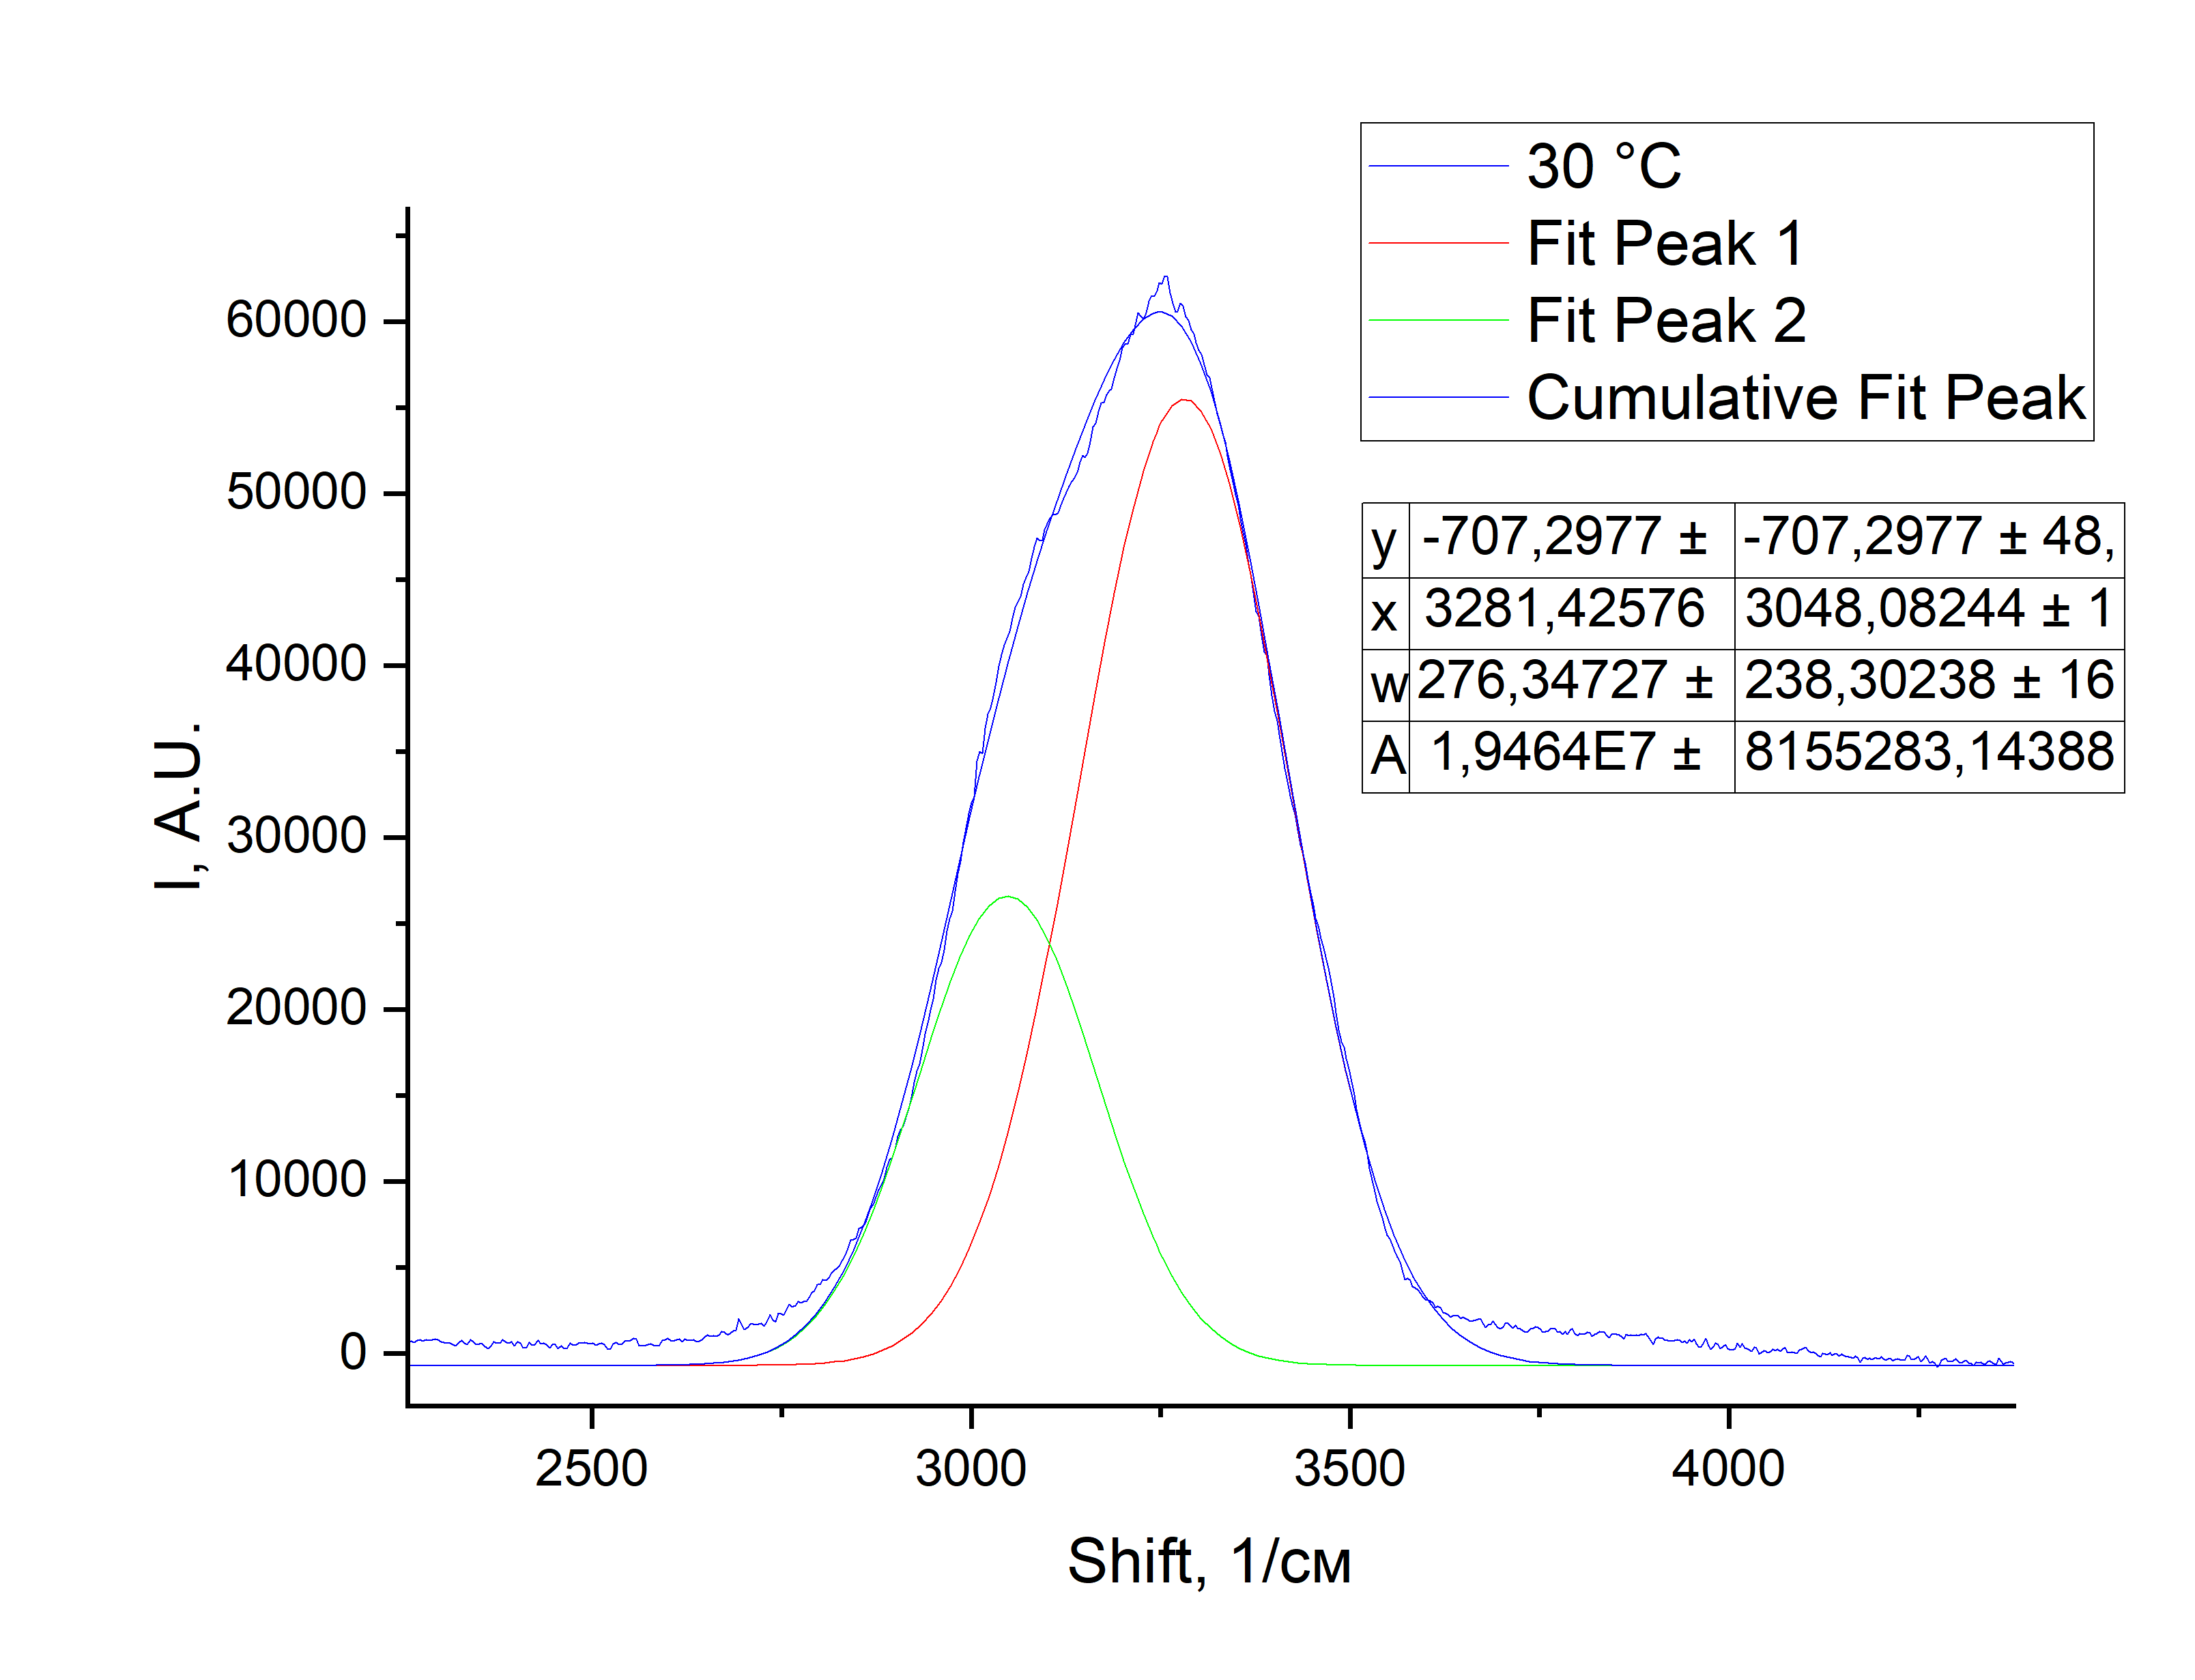
\includegraphics[width=\linewidth]{Images/Вода; 30.png}
                 \caption{Декомпозиция спектра КРС воды для $T = 30 \; ^{\circ}C$}
                  \endminipage
\end{figure}

\begin{figure}[!htb]
                \minipage{0.45\textwidth}
                 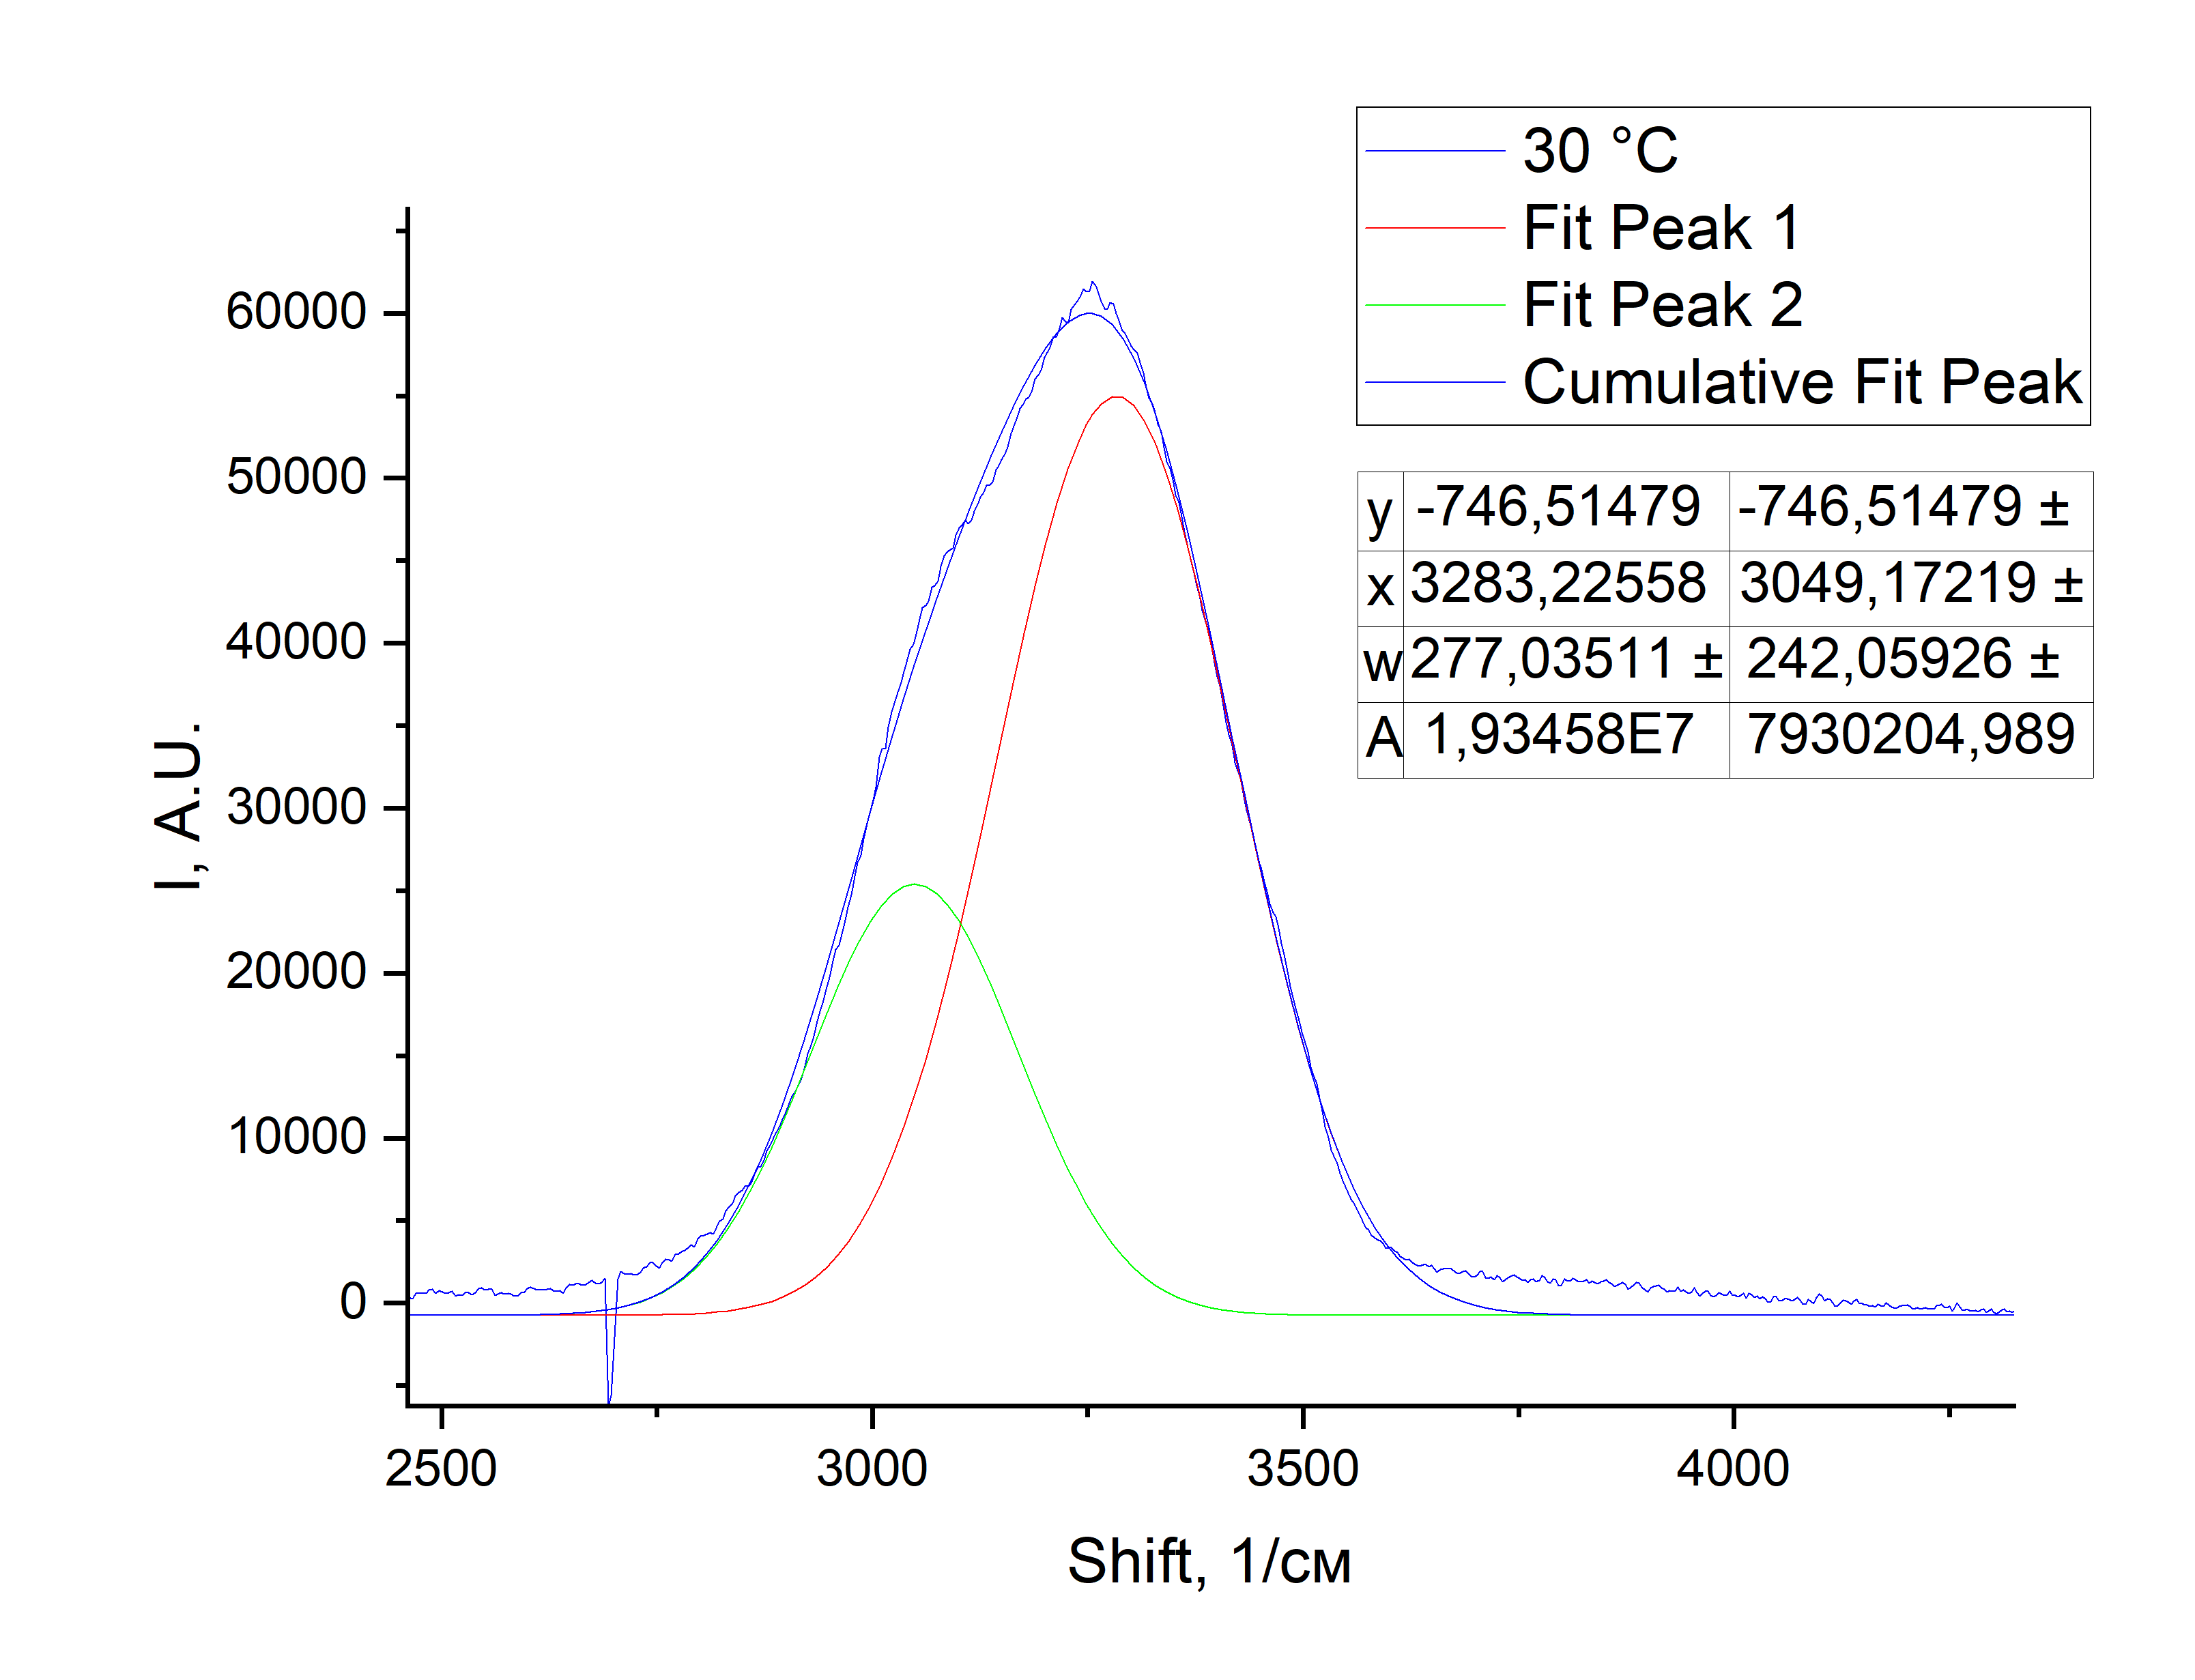
\includegraphics[width=\linewidth]{Images/Вода; 40.png}
                 \caption{Декомпозиция спектра КРС воды для $T = 40 \; ^{\circ}C$}
                  \endminipage\hfill
                \minipage{0.45\textwidth}
                 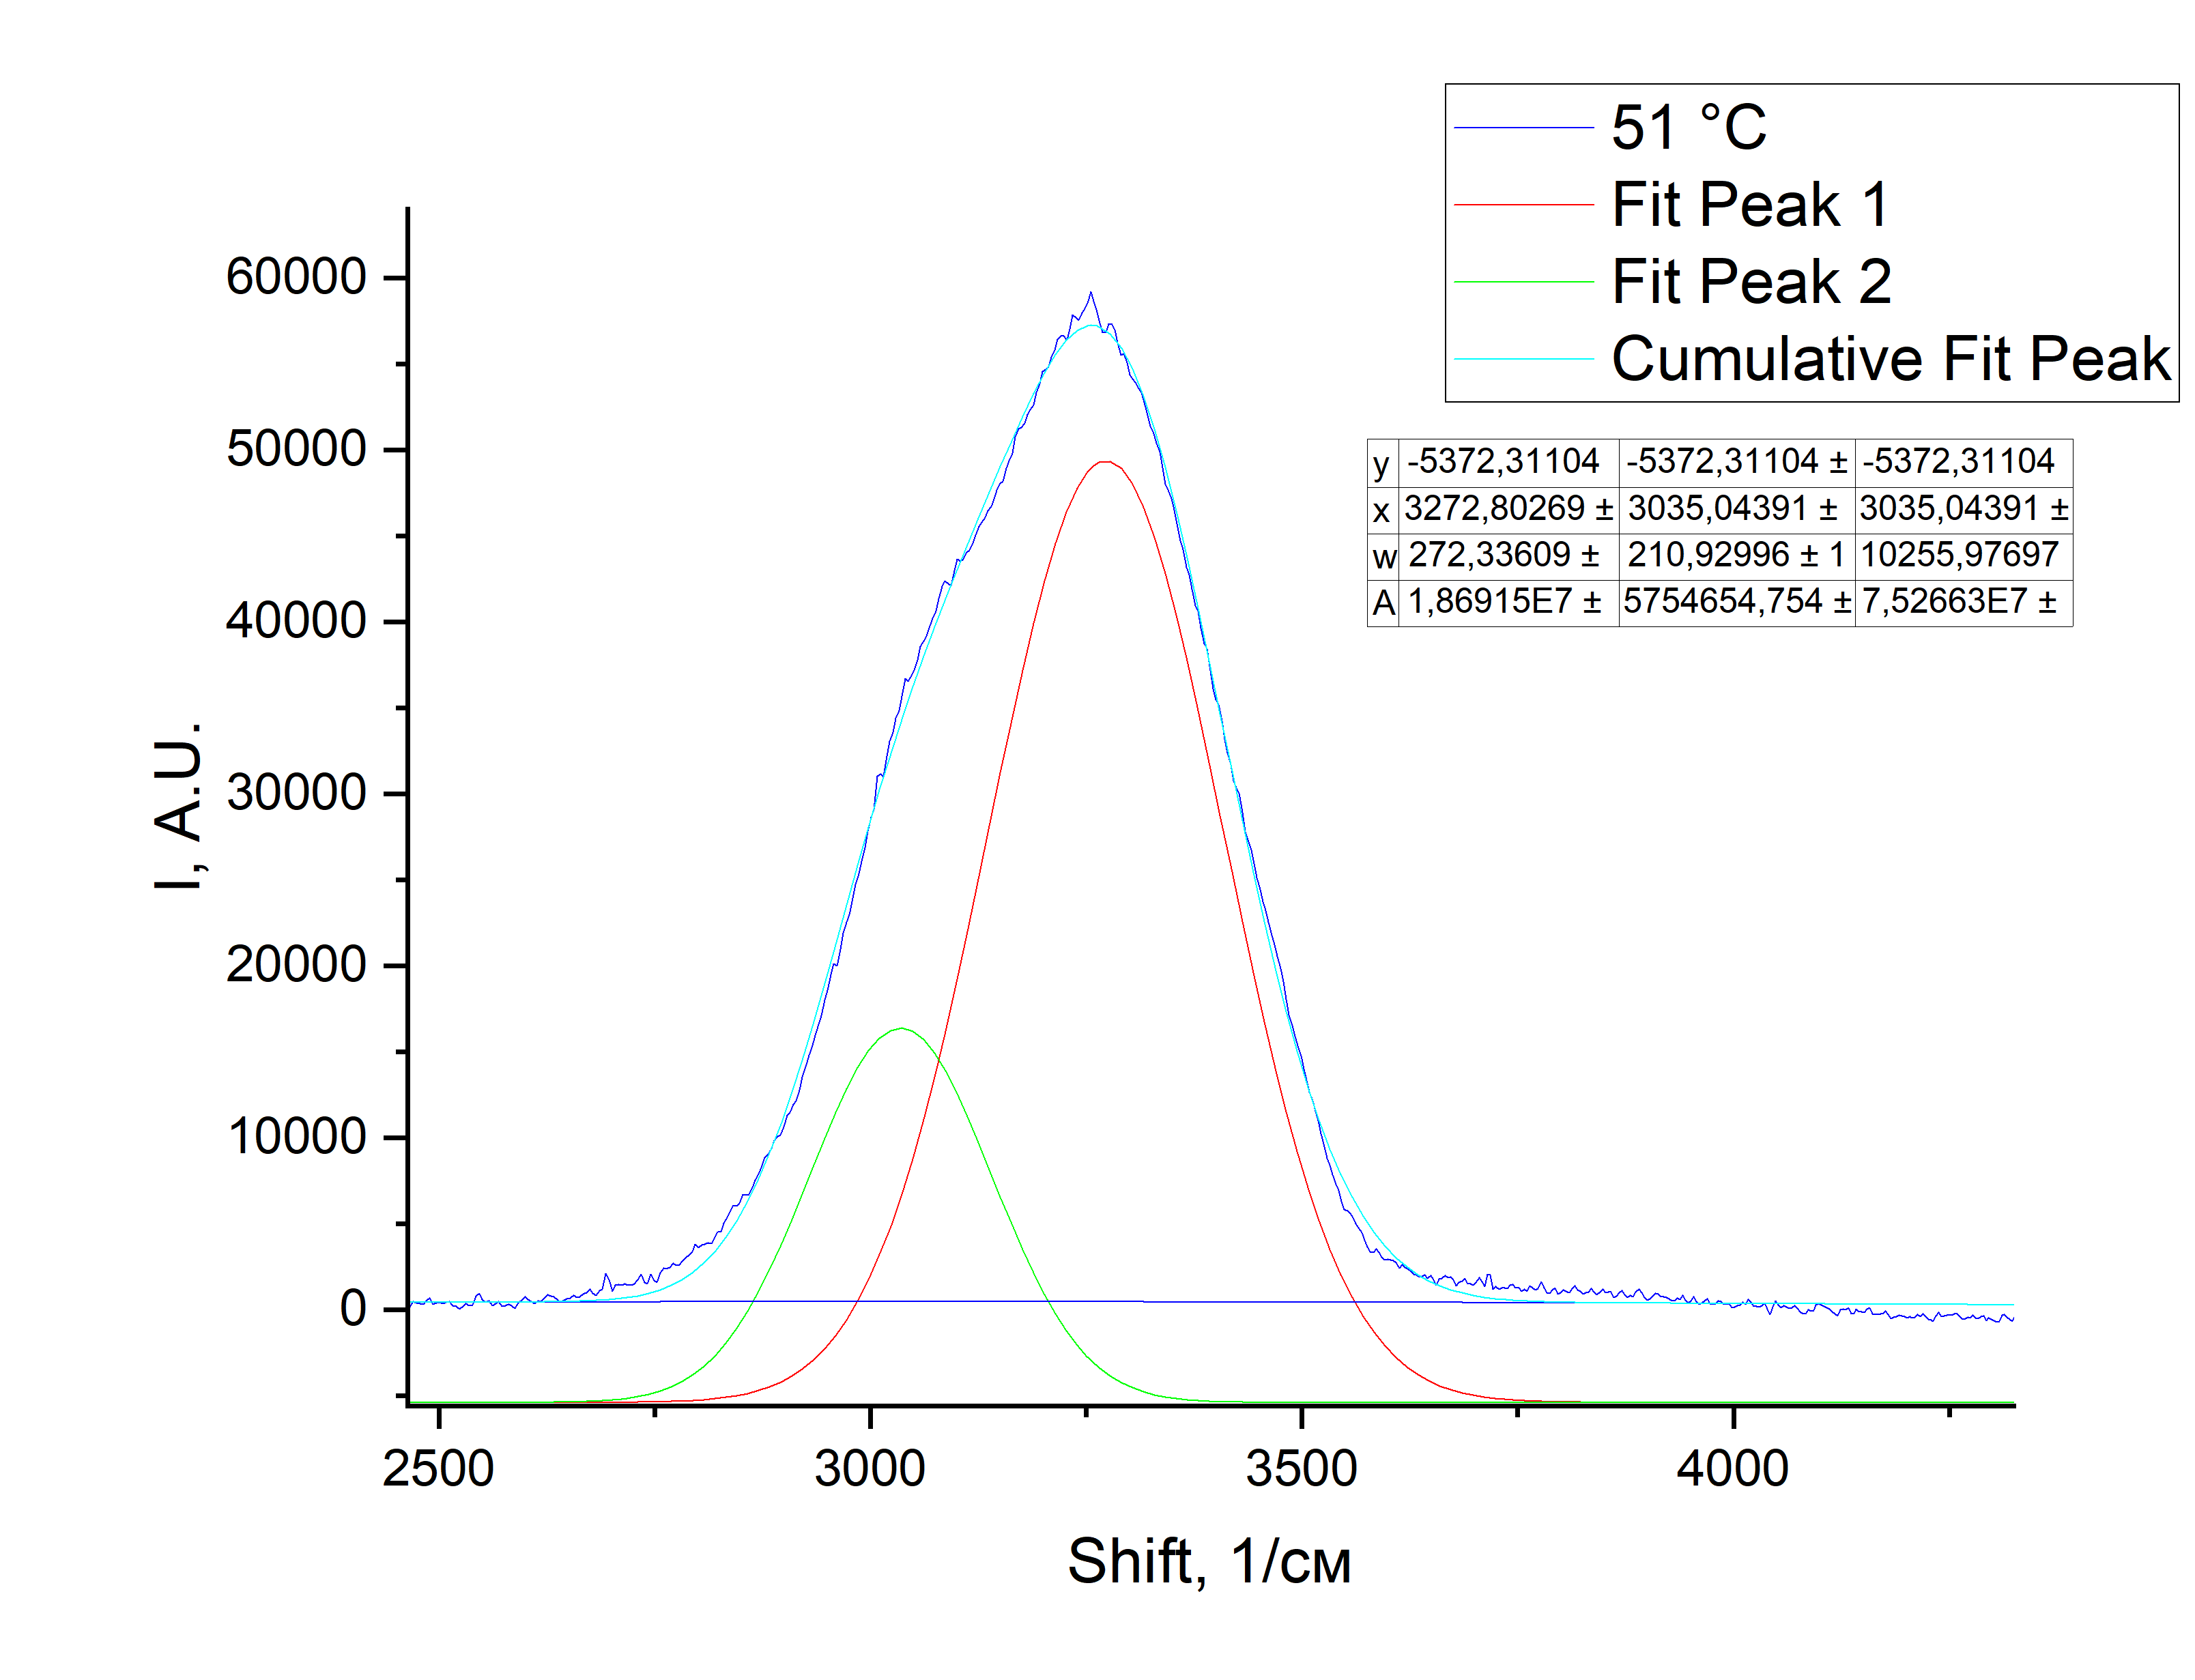
\includegraphics[width=\linewidth]{Images/Вода; 51.png}
                 \caption{Декомпозиция спектра КРС воды для $T = 51 \; ^{\circ}C$}
                  \endminipage
\end{figure}

\begin{figure}[!htb]
                \minipage{0.45\textwidth}
                 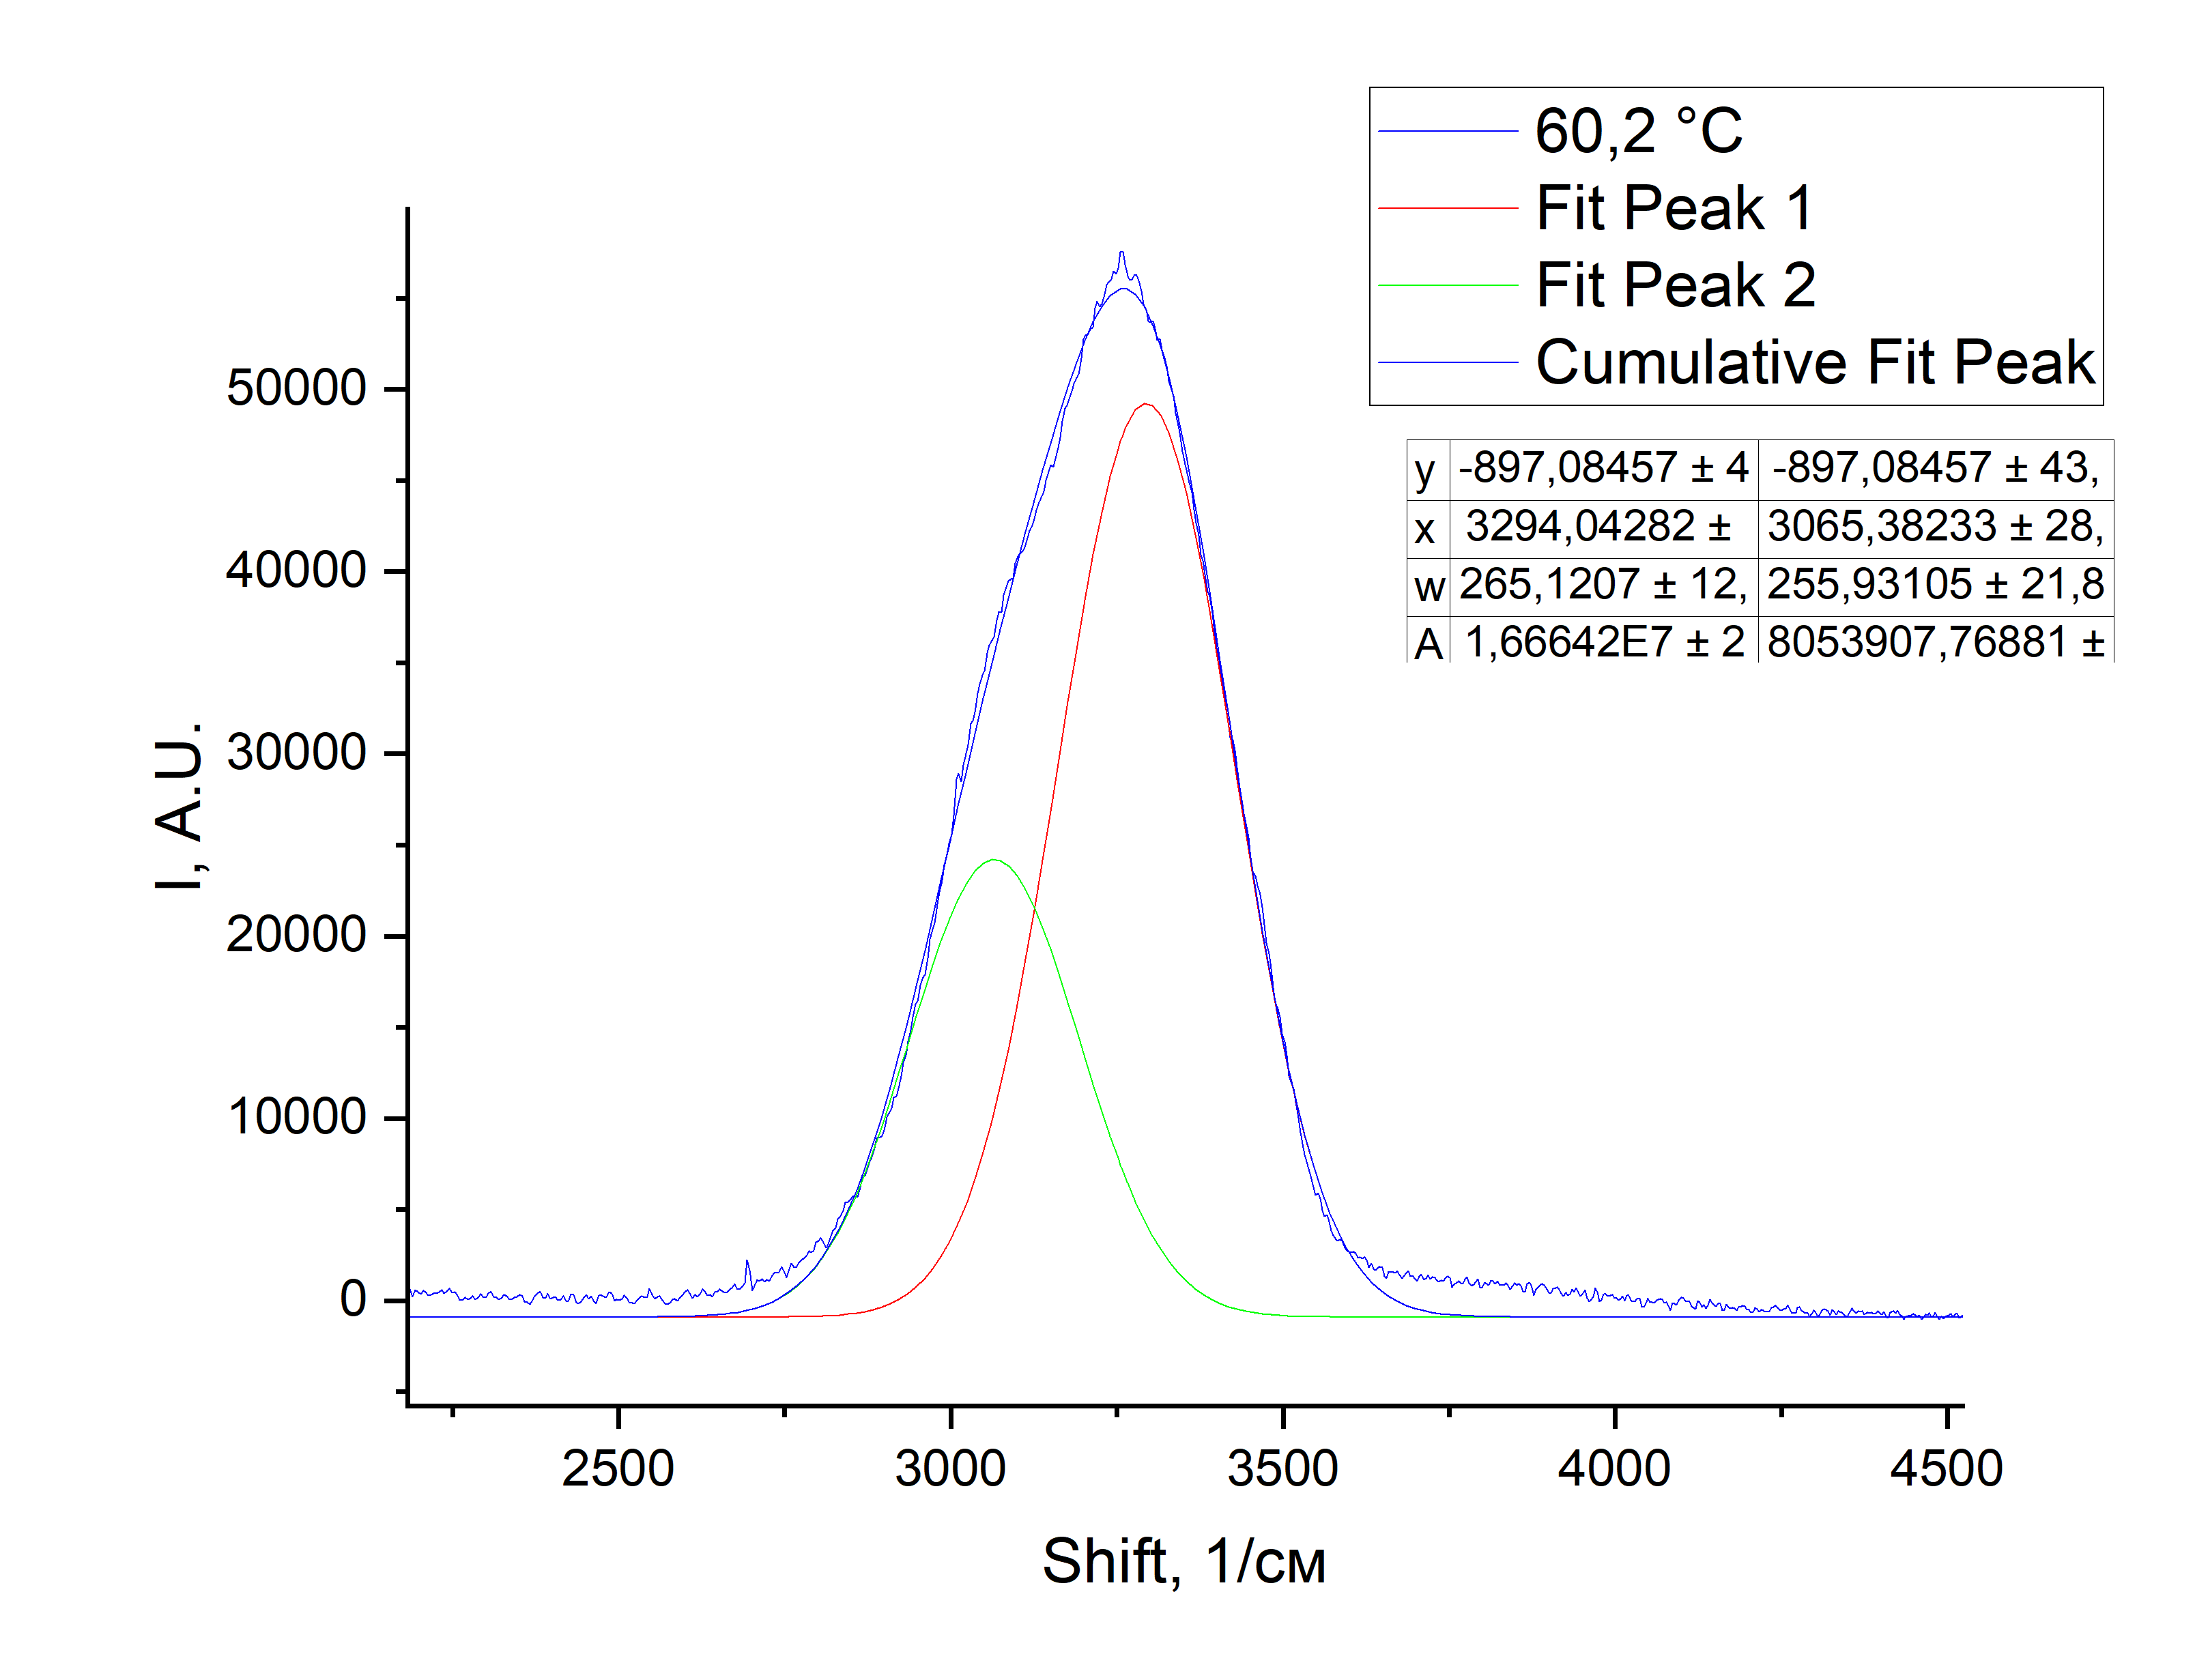
\includegraphics[width=\linewidth]{Images/Вода; 60,2.png}
                 \caption{Декомпозиция спектра КРС воды для $T = 60,2\; ^{\circ}C$}
                  \endminipage\hfill
                \minipage{0.45\textwidth}
                 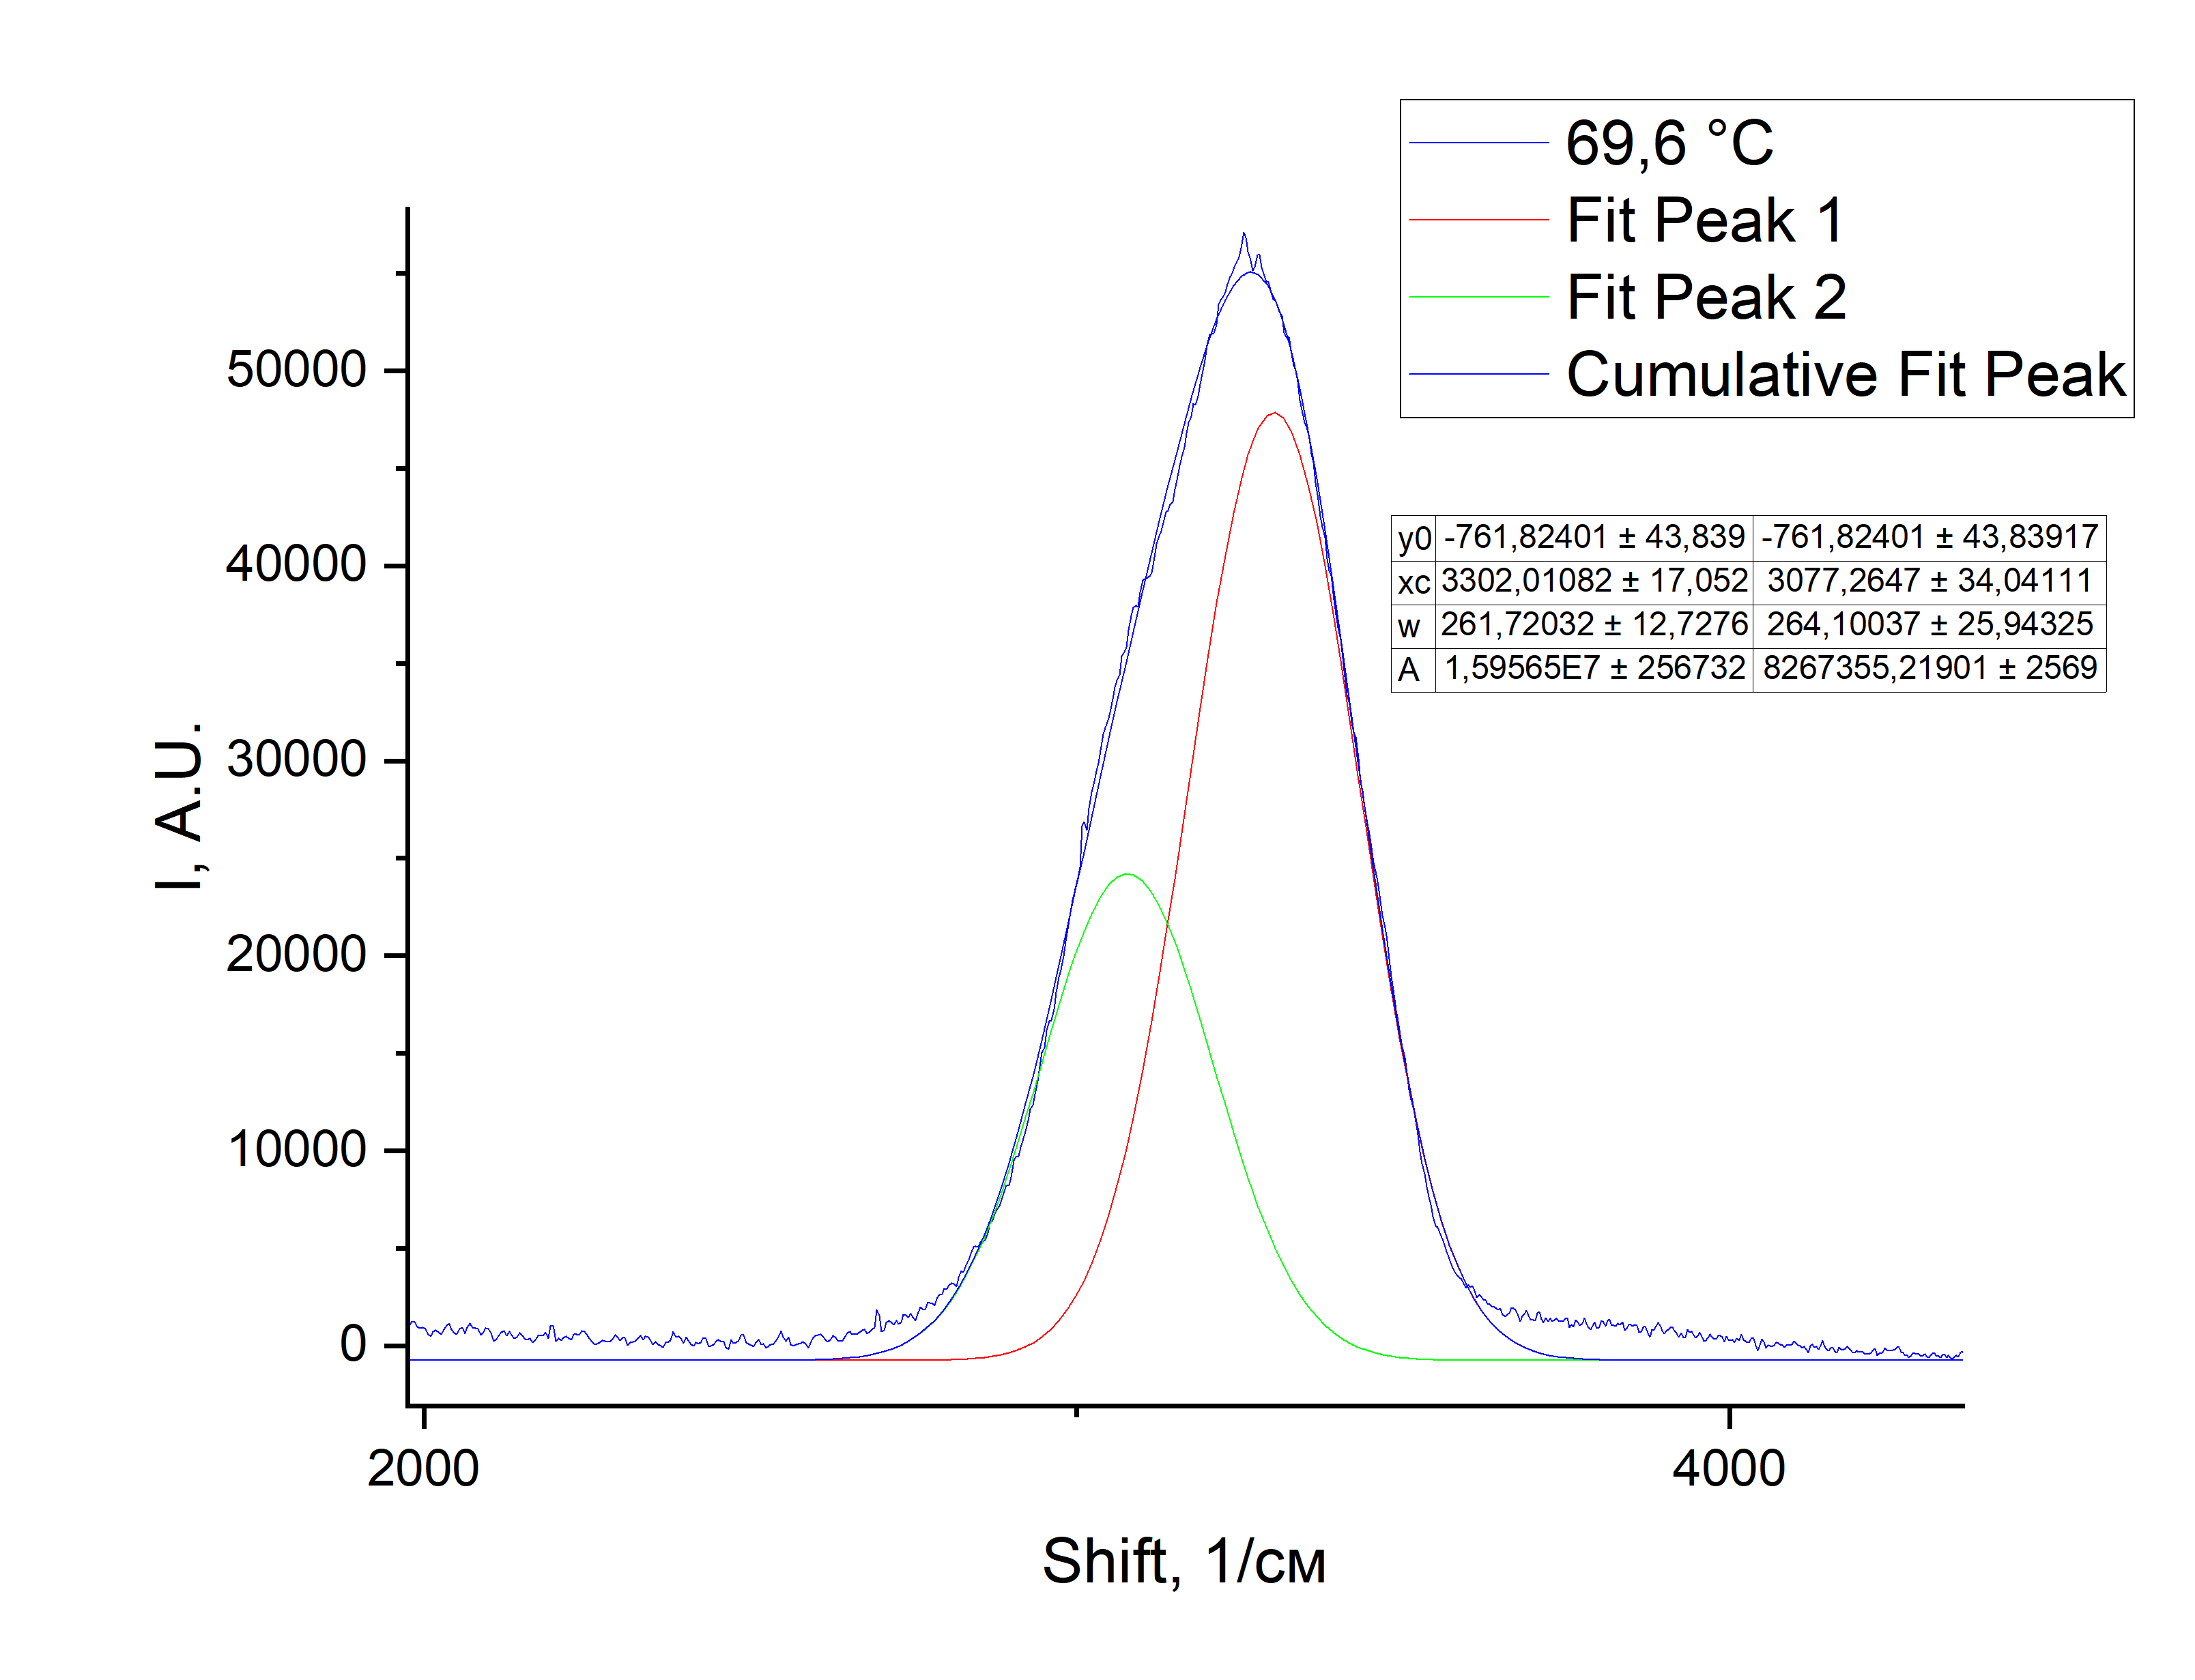
\includegraphics[width=\linewidth]{Images/Вода; 69,6.png}
                 \caption{Декомпозиция спектра КРС воды для $T = 69,6 \; ^{\circ}C$}
                  \endminipage
\end{figure}

\begin{figure}[h!]
\centering
    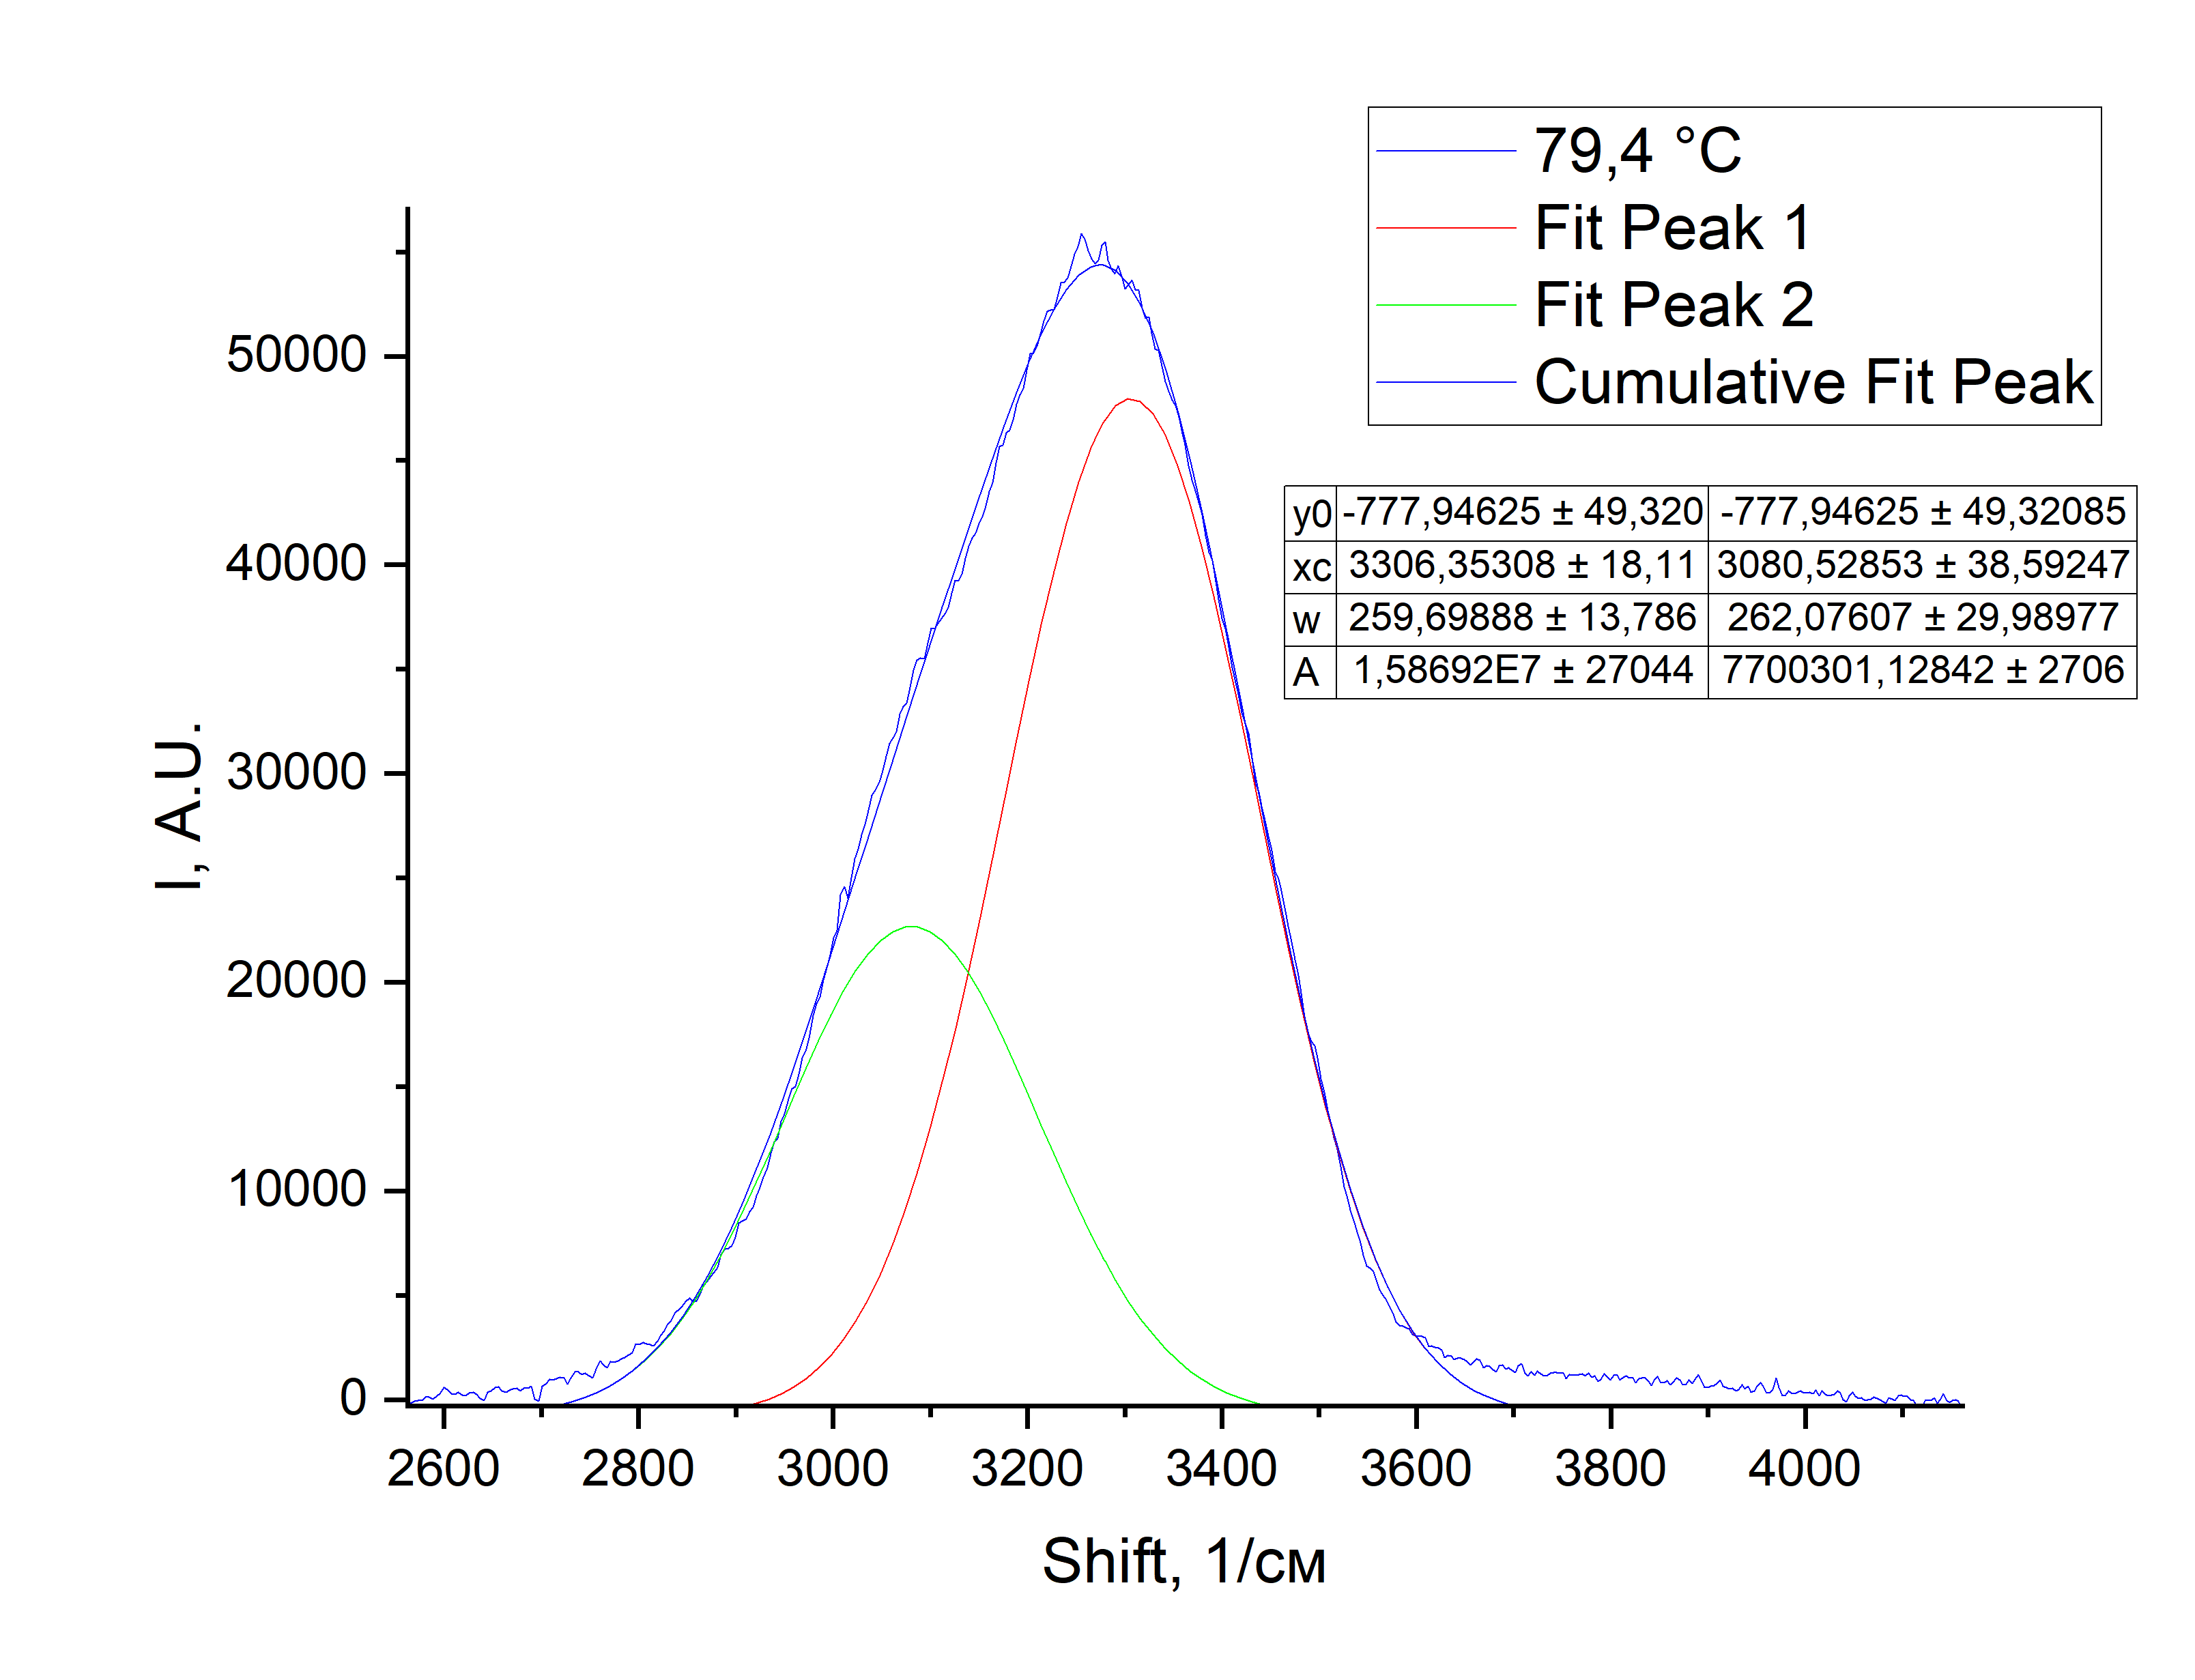
\includegraphics[width=0.6\linewidth]{Images/Вода; 79,4.png}
    \caption{Декомпозиция спектра КРС воды для $T = 79,4\; ^{\circ}C$}
\end{figure}
\end{document}
